\documentclass[a4paper,12pt, oneside]{book}

% \usepackage{fullpage}
\usepackage[italian]{babel}
\usepackage[utf8]{inputenc}
\usepackage{amssymb}
\usepackage{amsthm}
\usepackage{graphics}
\usepackage{amsfonts}
\usepackage{listings}
\usepackage{amsmath}
\usepackage{amstext}
\usepackage{engrec}
\usepackage{rotating}
\usepackage{verbatim}
\usepackage[safe,extra]{tipa}
%\usepackage{showkeys}
\usepackage{multirow}
\usepackage{hyperref}
\usepackage{microtype}
\usepackage{fontspec}
\usepackage{enumerate}
\usepackage{braket}
\usepackage{marginnote}
\usepackage{pgfplots}
\usepackage{cancel}
\usepackage{polynom}
\usepackage{booktabs}
\usepackage{enumitem}
\usepackage{framed}
\usepackage{pdfpages}
\usepackage{pgfplots}
\usepackage{algorithm}
% \usepackage{algpseudocode}
\usepackage[cache=false]{minted}
\usepackage{mathtools}
\usepackage[noend]{algpseudocode}

\usepackage{tikz}\usetikzlibrary{er}\tikzset{multi  attribute /.style={attribute
    ,double  distance =1.5pt}}\tikzset{derived  attribute /.style={attribute
    ,dashed}}\tikzset{total /.style={double  distance =1.5pt}}\tikzset{every
  entity /.style={draw=orange , fill=orange!20}}\tikzset{every  attribute
  /.style={draw=MediumPurple1, fill=MediumPurple1!20}}\tikzset{every
  relationship /.style={draw=Chartreuse2,
    fill=Chartreuse2!20}}\newcommand{\key}[1]{\underline{#1}}
  \usetikzlibrary{arrows.meta}
  \usetikzlibrary{decorations.markings}
  \usetikzlibrary{arrows,shapes,backgrounds,petri}
\tikzset{
  place/.style={
        circle,
        thick,
        draw=black,
        minimum size=6mm,
    },
  transition/.style={
    rectangle,
    thick,
    fill=black,
    minimum width=8mm,
    inner ysep=2pt
  },
  transitionv/.style={
    rectangle,
    thick,
    fill=black,
    minimum height=8mm,
    inner xsep=2pt
    }
  } 
\usetikzlibrary{automata,positioning}
\usepackage{fancyhdr}
\pagestyle{fancy}
\fancyhead[LE,RO]{\slshape \rightmark}
\fancyhead[LO,RE]{\slshape \leftmark}
\fancyfoot[C]{\thepage}
\usepackage[usenames,dvipsnames]{pstricks}
\usepackage{epsfig}
\usepackage{pst-grad} % For gradients
\usepackage{pst-plot} % For axes
\usepackage[space]{grffile} % For spaces in paths
\usepackage{etoolbox} % For spaces in paths
\makeatletter % For spaces in paths
\patchcmd\Gread@eps{\@inputcheck#1 }{\@inputcheck"#1"\relax}{}{}
\makeatother

\title{Architetture Dati}
\author{UniShare\\\\Davide Cozzi\\\href{https://t.me/dlcgold}{@dlcgold}}
\date{}

\pgfplotsset{compat=1.13}
\begin{document}
\maketitle

\definecolor{shadecolor}{gray}{0.80}
\setlist{leftmargin = 2cm}
\newtheorem{teorema}{Teorema}
\newtheorem{definizione}{Definizione}
\newtheorem{esempio}{Esempio}
\newtheorem{corollario}{Corollario}
\newtheorem{lemma}{Lemma}
\newtheorem{osservazione}{Osservazione}
\newtheorem{nota}{Nota}
\newtheorem{esercizio}{Esercizio}
\algdef{SE}[DOWHILE]{Do}{doWhile}{\algorithmicdo}[1]{\algorithmicwhile\ #1}
\tableofcontents
\renewcommand{\chaptermark}[1]{%
  \markboth{\chaptername
    \ \thechapter.\ #1}{}}
\renewcommand{\sectionmark}[1]{\markright{\thesection.\ #1}}
\newcommand{\floor}[1]{\lfloor #1 \rfloor}
\newcommand{\MYhref}[3][blue]{\href{#2}{\color{#1}{#3}}}%
\chapter{Introduzione}
\textbf{Questi appunti sono presi a lezione. Per quanto sia stata fatta
  una revisione è altamente probabile (praticamente certo) che possano
  contenere errori, sia di stampa che di vero e proprio contenuto. Per
  eventuali proposte di correzione effettuare una pull request. Link: }
\url{https://github.com/dlcgold/Appunti}.\\
\chapter{Sistemi centralizzati}
\begin{definizione}
  Un \textbf{DBMS (\textit{DataBase Management System})} è un sistema, ovvero un
  software, in grado di gestire collezioni di dati che siano:
  \begin{itemize}
    \item \textit{grandi}, ovvero di dimensioni maggiori della memoria centrale
    dei sistemi di calcolo usati (se ho a che fare con una quantità di dati non
    così grande e con un uso personale posso affidarmi ad una \textit{hashmap}
    piuttosto che ad un db)
    \item \textit{persistenti}, ovvero con un periodo di vita indipendente dalle
    singole esecuzioni dei programmi che le utilizzano e per molto tempo 
    \item \textit{condivise}, ovvero usate da diversi applicativi e diversi
    utenti (fattore che porta anche allo studio del carico di lavoro,
    \textit{workload}). L'accesso può essere sia \textit{in scrittura} che
    \textit{in lettura} (ovviamente anche entrambi) a seconda del caso. SI
    pongono quindi problemi di concorrenza e sicurezza
    \item \textit{affidabili}, sia resistente dal punto di vista hardware (un
    guasto non deve farmi perdere i dati) che dal punto di vista della sicurezza
    informatica. Le transazioni devono essere quindi \textbf{atomiche} (o tutto
    o niente) e \textbf{definitive} (che non verranno più dimenticate). Il
    software può cambiare mentre i dati no
  \end{itemize}
\end{definizione}
A livello di architettura per un \textit{sistema centralizzati} si hanno:
\begin{itemize}
  \item uno o più \textit{storage} per memorizzare i dati, a loro volta su uno o
  più file del \textit{file system}
  \item il \textit{DBMS}, il componente software che funge da componente logico
  \item diverse applicazioni che elaborano i dati provenienti dal db
  (\textit{lettura}) ed eventualmente scrivono dati sullo stesso
  (\textit{scrittura})
  \item il \textbf{DBA (\textit{DataBase Administrator})} che tramite riga di
  comando o GUI si occupa di manutenzione, sicurezza, ottimizzazione etc$\ldots$
  del DBMS 
\end{itemize}
L'\textit{architettura dati} di un DBMS è definita dall'ente \textit{ANSI/SPARC}
e è a tre livelli:
\begin{enumerate}
  \item diversi \textbf{schemi esterni}, porzioni di db messi a disposizione per
  le varie applicazioni
  \item uno \textbf{schema logico (o concettuale)}, che fa riferimento al
  \textit{modello relazionale} dei dati ed è indipendente dalla tecnologia
  usata. Avendo un unico schema logico si ha un'unica semantica (perlomeno a
  livello astratto). Si ha unica base di dati, quindi un unico insieme di record
  interrogati e aggiornati da tutti gli utenti. Non si ha nessuna forma di
  eterogeneità concettuale 
  \item uno \textbf{schema fisico}, che fa riferimento alla tecnologia usata per
  implementare le tabelle per salvare i dati. Si ha un'unica rappresentazione
  fisica dei dati e quindi nessuna distribuzione e nessuna eterogeneità fisica
\end{enumerate}
\textit{Un unico schema fisico è collegato ad un unico schema logico.}\\
Inoltre si hanno:
\begin{itemize}
  \item un \textbf{unico linguaggio di interrogazione} e quindi un'unica
  modalità di accesso ai dati
  \item un unico sistema di gestione per accesso, aggiornamento e gestione per
  la transazioni e le interrogazioni
  \item un'unica modalità di ripristino in caso d'emergenza
  \item un unico amministratore dei dati
  \item \textbf{nessuna autonomia gestionale}
\end{itemize}
Per il discorso della persistenza dei dati si ha necessità di una memoria
secondaria dove il DBMS salva le strutture dati, studiando un modo efficiente di
trasferimento dei dati nel \textit{buffer} in memoria centrale. Il
\textit{buffer} è un'area di memoria (o meglio un componente software) nella
memoria centrale che cerca, tramite una logica di ``vicinanza'', di mettere i
dati della memoria secondaria in quella centrale. Si usa il \textbf{principio di
  località}.\\
A causa degli accessi condivisi al db si hanno problemi di \textbf{concorrenza},
avendo accesso multi-utente alla stessa dei dati condivisa, accesso che
necessità anche di meccanismi di \textbf{autorizzazione}. In merito alla
concorrenza si ha che le transazioni sono corrette se \textbf{seriali} (ordinate
temporalmente) ma questo non è sempre applicabile e quindi si deve stabilire un
\textit{controllo della concorrenza}.\\
Per accedere ai dati di un db si hanno le \textbf{query
  (\textit{interrogazioni})} che fanno parte del modello logico a cui si
interfaccia l'utente. Essendo i dati nelle memorie secondarie bisogna cercare un
modo di rendere gli accessi performanti, in primis tramite opportune strutture
fisiche in quanto e strutture logiche non sarebbero efficienti in memoria
secondaria. Bisogna fare in modo che gli accessi alla memoria secondaria siano
il più limitati possibili e quindi bisogna ottimizzare l'esecuzione delle query.
Ovviamente una scansione lineare delle tabelle sarebbe troppo dispendiosa con
tabelle grosse, ricordando che i file sono ad accesso sequenziale. Inoltre un
ipotetico \textit{join} tra tabelle renderebbe ancora più complesso l'accesso,
soprattutto se \textit{full-join}.\\
Per poter garantire tutto ciò che è stato detto l'architettura del DBMS deve
essere organizzata in termini di \textit{funzionalità cooperanti}:
\begin{itemize}
  \item un \textbf{query compiler} che prende una query in SQL e la traduce con
  un compilatore
  \item un \textbf{gestore di interrogazioni e aggiornamenti} che trasforma le
  query in SQL in algebra relazionale facendo operazioni di ottimizzazione
  \item un \textbf{gestore dei metodi di accesso} per permettere il passaggio
  tra file e tabelle passando dal \textbf{gestore del buffer} e il
  \textbf{gestore della memoria secondaria} dove i dati non sono in forma
  tabellare ma di file e pagine
  \item un \textbf{DDL compiler}, dove DDL sta per Data Description Language,
  che si occupa dei comandi del DBA
  \item un \textbf{gestore della concorrenza}, che garantisce il controllo della
  concorrenza
  \item un \textbf{gestore dell'affidabilità}, che garantisce che un dato non
  vada perso
  \item un \textbf{gestore delle transazioni}
\end{itemize}
Gli ultimi quattro entrano in uso specialmente in fase di scrittura.\\
\textbf{Tutto deve essere veloce!}\\
In un sistema distribuito la parte di query compiler, gestore delle
interrogazioni, gestore delle transazioni e gestore della concorrenza resta
invariato mentre il resto cambia drasticamente (in quanto i dati sono
distribuiti) dovendo gestire diversamente l'accesso ai dati e la sua
sicurezza. Bisogna gestire anche come i vari nodi devono interagire coi dati.
\section{Ottimizzazione delle query}
Ottimizzare le query è tutt'altro che banale.\\
Il primo step è il \textbf{parsing}, che stabilisce se la query è sensata dal
punto di vista sintattico e se i vari nomi di tabelle e attributi sono coerenti
con lo schema. Per questo ultimo aspetta ci si appoggia al \textbf{Data
  Catalog}, un particolare db che contiene informazioni sui vari database, in
primis sui vari nomi delle tabelle e per ciascuna sui nomi di ogni attributo. SI
ha quindi una soluzione per gestire i \textit{metadati}. Il parser effettua
un'analisi lessicale, per la sintattica e la semantica, usando il dizionario e
l a traduzione in algebra relazionale, producendo un \textbf{query tree}. Si
calcola anche un \textbf{query plan logico}, utilizzando regole sintattiche di
buon senso, per capire cosa fare prima (per esempio se fare prima una
\textit{select} o un \textit{join}) per ottenere il risultato corretto nel minor
tempo possibile (prima di fare una \textit{join} magari seleziono prima una
sottotabella con i dati potenzialmente utili, togliendo quelli sicuramente
inutili$\ldots$ magari quel \textit{join} può anche essere evitato). La query
viene quindi rappresentata come un albero dove e foglie corrispondono alle
strutture dati logiche, ovvero le tabelle. I nodi interni sono invece le varie
\textbf{operazioni algebriche (\textit{select, join, proiezione, prodotto
    cartesiano} e \textit{operazioni insiemistiche})}.
\newpage
\begin{esempio}
  Vediamo una query:
  \begin{minted}{sql}
    SELECT Pnumber, Dnum, Lname, Address, Bdate
    FROM Project P, Dept D, Emp E
    Where P.dnum=D.dnumber and E.ssn = D.mgrssn
    and P.location = 'Stafford'
  \end{minted}
  che produce:
  \begin{center}
    \psscalebox{1.0 1.0} % Change this value to rescale the drawing.
    {
      \begin{pspicture}(0,-2.36)(10.7,2.36)
        \rput[bl](4.0,2.1249022){$\pi$ Pnumber, Dnum, Lname, Address, Bdate}
        \rput[bl](5.6,0.9249023){join mgrssn=ssn}
        \rput[bl](2.0,0.124902345){join dnum=dnumber}
        \rput[bl](8.4,0.124902345){emp}
        \rput[bl](0.0,-1.0750977){$\sigma$ plocation='stafford'}
        \rput[bl](6.4,-1.0750977){dept}
        \rput[bl](1.6,-2.2750976){project}
        \psline[linecolor=black, linewidth=0.04, arrowsize=0.05291667cm
        2.0,arrowlength=1.4,arrowinset=0.0]{<-}(6.8,1.3249023)(6.8,2.1249022)
        \psline[linecolor=black, linewidth=0.04, arrowsize=0.05291667cm
        2.0,arrowlength=1.4,arrowinset=0.0]{<-}(8.8,0.52490234)(8.4,0.9249023)
        \psline[linecolor=black, linewidth=0.04, arrowsize=0.05291667cm
        2.0,arrowlength=1.4,arrowinset=0.0]{<-}(5.2,0.52490234)(6.0,0.9249023)
        \psline[linecolor=black, linewidth=0.04, arrowsize=0.05291667cm 2.0,
        arrowlength=1.4,arrowinset=0.0]{<-}(3.6,-0.67509764)(3.6,0.124902345)
        \psline[linecolor=black, linewidth=0.04, arrowsize=0.05291667cm 2.0,
        arrowlength=1.4,arrowinset=0.0]{<-}(6.4,-0.67509764)(4.8,0.124902345)
        \psline[linecolor=black, linewidth=0.04, arrowsize=0.05291667cm
        2.0,arrowlength=1.4,arrowinset=0.0]{<-}(2.4,-1.8750976)(2.4,-1.0750977)
      \end{pspicture}
    }
  \end{center}
  ma l'ottimizzatore va oltre (magari invertendo i \textit{where} etc$\ldots$)
  con un query plan più efficiente che permette di cambiare automaticamente le
  query in altre più efficienti.\\
\end{esempio}
Si ha un db chiamato \textbf{Statistics} che contiene statistiche sulla storia
delle query nonché altre informazioni sui dati. L'uso di tale db permette di
ottimizzare le query.\\
Solo dopo questo processo si ha la trasformazione delle tabelle logiche in
strutture fisiche e metodi di accesso alla memoria e la trasformazione delle
operazioni algebriche nelle loro implementazioni sulle strutture fisiche. Per la
trasformazione si usano proprietà algebriche e una stima dei costi delle
operazioni fondamentali per diversi metodi di accesso (in poche parole le regole
della ricerca operativa). L'ottimizzazione ha complessità \textbf{esponenziale}
e quindi si introducono approssimazioni basate su euristiche, usando
un'\textbf{alberatura di costi} usando la tecnica del \textbf{Branch\&Bound}.
\section{Transazioni}
Una \textbf{transazione} è l'insieme di istruzioni di accesso in lettura e
scrittura ai dati, istruzioni eventualmente inserite in un linguaggio di
programmazione. Una transazione gode di proprietà che garantiscono la corretta
esecuzione anche in ambito di concorrenza e sicurezza, tanto che sono
paradigmatiche del modello relazionale. Le transazioni iniziano con un
\textbf{begin-transaction} (a volte finiscono con \textit{end-transaction},
opzionale) e all'interno deve essere eseguito tra:
\begin{itemize}
  \item \textbf{commit work}, per terminare correttamente la lettura e/o
  scrittura 
  \item \textbf{rollback work}, per abortire la transazione
\end{itemize}
Un \textbf{sistema transazionale OLTP (\textit{OnLine Transaction Processing})}
è in grado di definire ed eseguire transazioni per conto di un certo numero di
applicazioni concorrenti anche alto. 
\begin{esempio}
  Vediamo un esempio di transazione (esempio di addebito su un conto corrente e
  accredito su un altro):
  \begin{minted}{sql}
    start transaction;
    update ContoCorrente
      set Saldo = Saldo + 10 where
      NumConto = 12202;
    update ContoCorrente
      set Saldo = Saldo – 10 where
      NumConto = 42177;
    commit work;
  \end{minted}
  oppure, con anche la verifica che ci siano ancora soldi dopo il prelievo (con
  eventuale aborto):
  \begin{minted}{sql}
    start transaction;
    update ContoCorrente
      set Saldo = Saldo + 10 where
      NumConto = 12202;
    update ContoCorrente
      set Saldo = Saldo – 10 where
      NumConto = 42177;
    select Saldo into A
      from ContoCorrente
      where NumConto = 42177;
    if (A >= 0) then commit work
    else rollback work;
  \end{minted}
  Il controllo può essere fatto a posteriori grazie al rollback che permette di
  ``dimenticare'' tutte le operazioni precedenti
\end{esempio}
Le istruzioni commit work e rollback work possono comparire più volte
all'interno del programma ma esattamente una delle due deve essere eseguita. Si
ha un \textbf{approccio binario}.\\
Bisogna approfondire quindi le \textbf{unità di elaborazione} che hanno le
proprietà cosiddette \textit{ACID}:
\begin{itemize}
  \item \textbf{Atomicità}, ovvero una transazione è un'unità atomica di
  elaborazione. Non si può lasciare il db in uno ``stato 
  intermedio''. Un problema prima del commit cancella tutto le operazioni svolte
  (\textit{UNDO}) e un problema dopo il commit non deve avere conseguenze, se
  necessario vanno ripetute le operazioni (\textit{REDO}) 
  \item \textbf{Consistenza}, ovvero la transazione rispetta i vincoli di
  integrità (se lo stato iniziale è corretto lo è anche quello finale). Quindi
  se ci sono violazioni non devono restare alla fine (nel caso
  \textit{rollback})
  \item \textbf{Isolamento}, ovvero la transazione non risente delle altre
  transazioni concorrenti. Una transazione non espone i suoi stati intermedi
  evitando l'\textit{effetto domino} (si evita che il rollback di una
  transazione vada in cascata con le altre). L'esecuzione concorrente di una
  collezione di transazioni deve produrre un risultato che si potrebbe ottenere
  con una esecuzione sequenziale
  \item \textbf{Durabilità} (ovvero persistenza), ovvero gli effetti di una
  transazione andata in commit non vanno persi anche in presenza di guasti (a
  tal fine si sfrutta il \textbf{recovery manager}, che garantisce
  l'affidabilità, del DBMS)
\end{itemize}
\section{Gestore della concorrenza}
Il \textbf{gestore della concorrenza} permette di eseguire in parallelo più
operazioni.\\
Definiamo \textbf{schedule} come una sequenza di esecuzione di un insieme di
transazioni. Uno schedule è \textbf{seriale} se se una transazione  termina
prima che la successiva iniziale, altrimenti è \textbf{non seriale}. Qualora non
sia seriale si potrebbero avere problemi.\\
Si sfrutta quindi la \textbf{proprietà di isolamento} facendo in modo che ogni
transazione esegua come se non ci fosse concorrenza: \textit{un insieme di
  transazioni eseguite concorrentemente produce lo stesso risultato che
  produrrebbe una (qualsiasi) delle possibili esecuzioni sequenziali delle stesse
  transazioni allora si ha la proprietà di isolamento}.\\
Si ha quindi che uno schedule è serializzabile se l'esito della sua esecuzione è
lo stesso che si avrebbe con una qualsiasi sequenza seriale delle transazioni
contenute.\\
Si hanno quindi diversi algoritmi per il controllo della concorrenza secondo
varie tipologie:
\begin{itemize}
  \item controllo basato su \textit{conflict equivalence}
  \item controllo di concorrenza basato su \textit{locks} \textit{(protocollo
    2PL o two phase locking, shared locks e gestione dei deadlock}). Il
  protocollo 2PL è usato nei DBMS dove per costruzione si hanno schedule
  serializzabili usando i lock per  bloccare l'accesso alla risorse da parte di
  una transazione fino a che una risorsa non sia rilasciata. Si hanno quindi i
  concetti di \textit{lock} e \textit{unlock} che garantiscono l'uso esclusivo
  di una risorsa e l'autorizzazione esclusiva dell'uso di una risorsa viene dato
  dal gestore delle transazioni. Si hanno delle \textbf{tabelle di lock}. Si ha
  che, in ogni transazione, tutte le richieste di \textit{lock} precedono tutti
  gli \textit{unlock} (che comunque devono essere fatti dopo l'operazione di
  \textit{commit}) 
  \item controllo di concorrenza basato su \textit{timestamps}
\end{itemize}
\chapter{Sistemi distribuiti relazionali}
Abbiamo visto nei sistemi centralizzati come ci fosse una sola base dati. In un
sistema distribuito abbiamo diversi \textbf{basi dati locali}, diverse
applicazioni su ogni nodo di elaborazione (dove ogni nodo condivide varie
informazioni) con gli utenti che accedono alle varie applicazioni. Questo tipo
di architettura prende il nome di \textbf{architettura shared nothing}, in
quanto i DBMS di ogni singola macchina sono autonome (anche di vendor diversi)
ma che lavorano insieme.\\
Un sistema distribuito permette non solo di avere dati ``distribuiti'' tra vari
nodi ma anche di ``duplicarne'' alcuni per diversi scopi, coi nodi collegati in
rete (addirittura si hanno soluzioni interamente distribuite nel cloud).\\
Confrontando un db distribuito con un multi-database (ovvero vari database
completi da ``unificare'') notiamo come entrambi
abbiano un'alta distribuzione, il primo una bassa eterogeneità (a differenza del
secondo, dove nei vari db potrei avere forte differenza di tipologia dei dati
contenuti). Si ha anche bassa autonomia nel caso si db distribuiti a differenza
del multi-database (dove ogni db è singolarmente autonomo).\\
Bisogna capire cosa distribuire. Si hanno diverse condizioni (che possono essere
presenti simultaneamente):
\begin{itemize}
  \item le applicazioni, fra loro cooperanti, risiedono su più nodi elaborativi
  \textbf{(elaborazione distribuita})
  \item l'archivio informativo è distribuito su più nodi (\textbf{base di dati
  distribuita}) 
\end{itemize}
La distribuzione si dice essere \textbf{ortogonale e trasparente} agli altri.\\
Capire cosa distribuire è una parte consistente dello studio di come costruire
un'architettura distribuita (magari frutto di situazioni particolari come la
``fusione'' di due sistemi a causa di un'acquisizione aziendale etc$\ldots$ dove
diverse logiche applicative e diverse strutture dati possono creare situazioni
molto pericolose).\\
Possiamo classificare i db distribuiti. Si ha innanzitutto che un \textbf{DBMS
Distribuito Eterogeneo Autonomo} è in generale una federazione di DBMS che
collaborano nel fornire servizi di accesso ai dati con livelli di
\textit{trasparenza} definiti (infatti le diversità tra db nei nodi vengono
``nascosti'' a vari \textit{livelli di trasparenza} per distribuzione,
eterogeneità e autonomia). Come abbiamo visto esiste l'esigenza di integrare a
posteriori vari db preesistenti (anche a causa di integrazione di nuovi
applicativi o nuove cooperazioni di processi) e questa situazione è spinta
dallo sviluppo della rete.\\
Possiamo quindi dividere i livello di federazione su tre categorie tra loro
ortogonali (ovvero indipendenti):
\begin{itemize}
  \item autonomia
  \item distribuzione
  \item eterogeneità
\end{itemize}
\subsubsection{Autonomia}
L'\textbf{autonomia} fa riferimento al grado di indipendenza tra i nodi e si
hanno diverse forme:
\begin{itemize}
  \item \textbf{autonomia di progetto}, il livello ``massimo'' dove ogni nodo ha
  un proprio modello dei dati e di gestione delle transazioni
  \item \textbf{autonomia di condivisione}, dove ogni nodo sceglie la porzione
  di dati da condividere ma condividendo con gli altri nodi lo schema comune
  \item \textbf{autonomia di esecuzione}, dove ogni nodo sceglie in che modo
  eseguire le transazioni
\end{itemize}
Si hanno quindi:
\begin{itemize}
  \item \textbf{DBMS Strettamente integrati} con nessuna autonomia, con dati
  logicamente centralizzati, un unico data manager per le transazioni
  applicative e vari data manager locali che non operano in modo autonomo ma
  eseguono le direttive centrali
  \item \textbf{DBMS semi-autonomi}, dove ogni data manager è autonomo ma
  partecipa a transazioni globali, dove una parte dei dati è condivisa e dove
  sono richieste modifiche architetturali  per poter fare parte della
  federazione
  \item \textbf{DBMS Peer to Peer} completamente autonomi, dove ogni DBMS lavora
  in completa autonomia ed è inconsapevole dell'esistenza degli altri  
\end{itemize}
\subsubsection{Distribuzione}
Per la\textbf{ distribuzione} dei dati si hanno 3 livelli classici:
\begin{itemize}
  \item \textbf{distribuzione client/server}, in cui la gestione dei dati è
  concentrata nei server, mentre i client forniscono l'ambiente applicativo e la
  presentazione
  \item \textbf{distribuzione Peer to Peer}, in cui non c'è distinzione tra
  client e server, e tutti i nodi del sistema hanno identiche funzionalità DBMS
  \item \textbf{nessuna distribuzione}
\end{itemize}
Le prime due possono anche non essere distinte.
\subsubsection{Eterogeneità}
L'\textbf{eterogeneità} può invece riguardare vari aspetti:
\begin{itemize}
  \item \textbf{modello dei dati} (relazionale, XML, object oriented (OO), json)
  \item \textbf{linguaggio di query} (diversi dialetti SQL, query by example,
  linguaggi di interrogazione OO o XML)
  \item \textbf{gestione delle transazione} (protocolli diversi per il gestore
  della concorrenza o per il recovery)
  \item \textbf{schema concettuale e logico} (concetti rappresentati in uno
  schema come attributo e in altri come entità)
\end{itemize}
Quindi si hanno vari tipi di DBMS:
\begin{itemize}
  \item \textbf{DBMS distribuito omogeneo (DDBMS)} quando si ha alta
  distribuzione ma non si hanno autonomia ed eterogeneità (gestiti solitamente
  dallo stesso vendor)
  \item \textbf{DBMS eterogeneo logicamente integrato (data warehouse)} quando
  si ha alta eterogeneità ma non si hanno distribuzione e autonomia
  \item \textbf{DBMS distribuiti eterogenei} quando si ha alta eterogeneità e
  distribuzione ma non autonomia 
  \item \textbf{DBMS federati distribuiti} quando si ha alta
  distribuzione, semi autonomia e non eterogeneità
  \item \textbf{DBMS distribuiti federati eterogenei} quando si ha alta
  distribuzione ed eterogeneità e semi autonomia
  \item \textbf{multi db MS}, totalmente autonomi ed eventualmente omogenei o
  eterogenei 
\end{itemize}
\textit{Si hanno molti altri sistemi in base alle 3 categorie}.\\
\section{DDBMS}
Parliamo di \textbf{DBMS distribuito omogeneo (\textit{DDBMS})}.\\
Studiamo uno schema in cui si passa da un sistema centralizzato ad un sistema
distribuito.\\
Si hanno due architetture di riferimento:
\begin{itemize}
  \item l'\textbf{architettura dati}
  \item l'\textbf{architettura funzionale}, ovvero l'insieme di tecnologie a
  supporto dell'architettura dati
\end{itemize}
Non avendo eterogeneità mantengo lo stesso schema di un DBMS centralizzato ma
distribuisco dati bisogna prendere lo schema centralizzato e aggiungere
componenti tra lo schema logico e lo schema fisico. Infatti non si avrà più un
solo schema logico e un unisco schema fisico ma tanti schemi logici e fisici
locali (ad ogni logico corrisponde un fisico). I vari schemi logici inoltre si
interfacciano con uno \textbf{schema logico globale}, i vari schemi logici
locali non sono quindi altro che delle \textit{viste} dello schema logico
globale. Questa organizzazione tra schemi logici locali e schema logico globale
è la cosiddetta \textbf{organizzazione LAV (\textit{Local As View})}. In ogni
caso il progettista interroga lo schema logico globale e saranno varie
tecnologie ad interrogare gli schemi logici locali (si fa una sorta di routing
delle query).\\
Per ciascuna funzione (come query processing, transaction manager etc$\ldots$)
si possono avere vari tipi di gestione:
\begin{itemize}
  \item centralizzata/gerarchica o distribuita
  \item con assegnazione statica o dinamica dei ruoli
\end{itemize}
\textit{Lo schema globale viene progettato prima degli schemi locali.}\\
Ovviamente cambia il \textbf{processo di progettazione} nel caso dei
DDBMS. Normalmente si ha un approccio \textit{top-down} per la progettazione,
con:
\begin{enumerate}
  \item analisi dei requisiti
  \item progettazione concettuale
  \item progettazione logica
  \item progettazione fisica
\end{enumerate}
ma questo tipo di progettazione va cambiato e quindi si introduce una nuova
fase e si cambiano le ultime due:
\begin{enumerate}
  \item analisi dei requisiti
  \item progettazione concettuale
  \item \textbf{progettazione della distribuzione}, per capire dove mettere i
  dati
  \item progettazione logica \textbf{locale}, che traduce dallo schema
  concettuale globale allo schema logico locale solo alcuni concetti
  \item progettazione fisica \textbf{locale}
\end{enumerate}
Si introduce il concetto di \textbf{portabilità}, ovvero la capacità di
eseguire le stesse applicazioni DB su ambienti runtime diversi (anche con SQL
diversi e differenti dallo standard). La portabilità è a \textit{compile-time}\\
Si ha anche il concetto di \textbf{interoperabilità} (tra vendors diversi),
ovvero la capacità di eseguire applicazioni che coinvolgono contemporaneamente
sistemi diversi ed eterogenei (con zero autonomia). A tal fine sono stati
introdotti dei \textit{middleware}, tra cui \textbf{ODBC} che si occupa
dell'accesso a dati di diversi vendor. ODBC, a livello architetturale, si pone
sopra il DBMS e da un'immagine indipendente da ciò che c'è sotto (funziona come
una sorta di \textit{driver}), trasformando tutto in una sorta di SQL
standard. Si hanno anche dei protocolli, come \textbf{X-Open Distributed
  Transaction Processing (\textit{DTP})} (che è una descrizione architetturale
abilitante il protocollo di esecuzione di transazioni distribuite), che
consentono di eseguire delle 
transazioni secondo una logica diversa. Questo protocollo stabilisce una serie
di API che vengono implementate da ogni singolo DBMS per offrire una
connettività standard (approccio molto usato per transazioni con vendor
diversi). Il protocollo funziona sia se si ha che fare con omogeneità che con
eterogeneità. \\
Si hanno altri approcci:
\begin{itemize}
  \item \textbf{basi dati parallele}, con incremento delle prestazione mediante
  parallelismo sia di storage devices che di processore (scalabilità
  orizzontale). Un esempio sono le \textbf{basi dati GRID}
  \item \textbf{basi dati replicate} dove si ha la
  replicazione della stessa informazione su diversi server per motivi di
  performance. Importanti per i temi della consistenza e della sicurezza
  \item \textbf{Data warehouses}, ovvero DBMS centralizzati, risultato
  dell'integrazione di fonti eterogenee, dedicati nel dettaglio alla gestione di
  dati per il supporto alle decisioni. Prevede la \textit{cristallizzazione} dei
  dati, acquisiti da varie sorgenti, creando un nuovo schema con la
  memorizzazione dei dati in formato nuovo (solitamente relazionale). Non usa un
  approccio LAV 
\end{itemize}
\subsection{Caratteristiche dei DDBMS}
Si hanno vari tipi di architetture DDBMS:
\begin{itemize}
  \item \textbf{shared-everything}, ad esempio \textit{SMP server}, dove il db
  management system e il disco sono in un unico nodo
  \item \textbf{shared-disk}, ad esempio \textit{Oracle RAC}, dove diversi db
  management systems 
  agiscono su una stessa \textbf{SAN (\textit{Storage Area Network})}, ovvero
  un'architettura dati di puro storage (con tanti dischi in raid). I vari db
  accedono ai dati secondo una certa regolazione. Viene distribuito il carico
  sui db ma si hanno problemi di concorrenza e hanno grandi problemi di
  scalabilità e costo economico
  \item \textbf{shared-nothing}, sempre più usati, dove ogni db management
  system ha il suo disco. È molto scalabile e, a patto di gestire la
  complessità, posso aggiungere nodi in modo illimitato (\textbf{scalabilità
    orizzontale}). Si presta molto all'ambiente cloud. Sono \textit{architetture
  federate}.
\end{itemize}
Vediamo quindi le proprietà generali di un DDBMS (facendo esplicito riferimento
alle architetture \textit{shared-nothing} per la loro scalabilità):
\begin{itemize}
  \item \textbf{località}, secondo il \textit{principio di località}, che
  garantisce un aumento di performances (nonché di sicurezza) tenendo i dati si
  trovano ``vicino'' 
  alle applicazioni che li utilizzano più frequentemente 
  \item \textbf{modularità}, permettendo di scalare orizzontalmente e
  permettendo modifiche a dati ed applicazioni a basso costo
  \item \textbf{resistenza ai guasti}
  \item \textbf{prestazioni ed efficienza}
\end{itemize}
Concentrandoci sulla \textbf{località} si ha che la partizione dei dati
corrisponde spesso ad una partizione naturale delle applicazioni e degli utenti.
I dati risiedono più vicino a dove vengono più usati ma possono comunque essere
raggiunti anche da lontano (\textit{globalmente}). Si cerca inoltre sempre di
più di spostare i dati verso le applicazioni (paradigma ribaltato nel caso di
\textit{big data}).\\
In merito alla \textbf{modularità} si nota come la distribuzione dinamica dei
dati si adatta meglio alle esigenze delle applicazioni (magari spostando solo
sottotabelle verso alcuni nodi etc$\ldots$, sia in modo trasparente rispetto
all'utente che altrimenti).\\
Parlando di \textbf{resistenza ai guasti} si ha una maggior fragilità a causa
delle unità che aumentano di numero ma si ha \textbf{ridondanza} e quindi
maggiore resistenza ai guasti di dati e applicazioni ridondate (\textit{fail
  soft}).\\
Discorso più interessante è da farsi sulle \textbf{prestazioni}. Ogni nodo in un
sistema shared-nothing gestisce db di dimensioni ridotte. Inoltre ogni nodo può
essere ottimizzato ad hoc ed è più semplice gestire e ottimizzare applicazioni
locali. Si ha inoltre distribuzione del carico totale e parallelismo  tra
transazioni locali che fanno parte di una stessa transazione distribuita (anche
se questo aspetta obbliga soluzioni di coordinamento e appesantisce il carico
sulla rete, che rischia di diventare un ``collo di bottiglia'').\\
I DDBMS hanno ovviamente \textbf{funzionalità} specifiche.\\
Ogni server ha buona capacità di gestire transazioni indipendentemente, anche se
le interazione distribuita tra server rappresentata un carico supplementare. Per
le interrogazioni si ha che le query arrivano dalle applicazioni e i risultati
dai server mentre per le transazioni le richieste transazionali arrivano dalle
applicazioni ma sono richiesti \textbf{dati di controllo} per il
coordinamento.\\’
La gestione della rete deve essere ottimizzata e serve uno studio sulla
distribuzione locale dei dati.\\
Ricapitolando si hanno le seguenti funzionalità specifiche:
\begin{itemize}
  \item \textbf{trasmissione} di query, transizioni, frammenti di db e dati di
  controllo tra i nodi
  \item \textbf{frammentazione, replicazione e trasparenza} (secondo vari
  livelli), fattori legati alla natura distribuita dei dati
  \item un \textbf{query processor} e un \textbf{query plan} per la previsione
  di una strategia globale accanto a strategie per le query locali. Si gestisce
  il passaggio tra schema logico globale e quelli locali. Chi esegue
  la query lo fa senza pensare alla frammentazione dei dati
  \item \textbf{controllo di concorrenza} tramite algoritmi distribuiti,
  fondamentale per gli accessi \textit{in scrittura}
  \item \textbf{strategie di recovery} e \textbf{gestione dei guasti}, sia in
  merito alla rete che all'hardware stesso
\end{itemize}
\subsection{Frammentazione e replicazione}
Si definisce \textbf{frammentazione} come la possibilità di allocare porzioni
(\textit{chunk}) diverse del db su nodi diversi.\\
Si definisce \textbf{replicazione} come la possibilità di allocare stesse
porzioni del db su nodi diversi.\\
Si definisce \textbf{trasparenza} come la possibilità per l'applicazione di
accedere ai dati senza sapere dove sono allocati (serve qualcosa che instradi le
query).
\subsubsection{frammentazione}
Esistono due tipi di frammentazione:
\begin{enumerate}
  \item \textbf{frammentazione orizzontale}, che prevede di prendere una tabella
  e frammentare in base alle righe (le prime $n$ da una parte, le seconde $m$
  dall'altra etc$\ldots$). Si mantiene quindi inalterato lo schema in quanto
  ottengo solamente delle tabelle più piccole in quanto pezzi. Per spezzare uso
  una \textit{select} (per la \textbf{selezione}) che selezioni ogni volta un
  certo ``blocco'' di tabella 
  \item \textbf{frammentazione verticale}, che consente di ridurre la
  dimensionalità della tabelle spezzandola in base alle colonne. In ogni nuova
  tabella però la prima colonna deve essere uguale alla prima della tabella
  originale (ovvero dove si ha la chiave primaria), questo per garantire che si
  possa ricomporre la tabella (e lo schema) originale (con operazioni di
  \textit{join}, o meglio un \textit{natural join}) e garantire la
  trasparenza. Anche in questo caso uso 
  una \textit{select} (per la \textbf{proiezione}) che selezioni ogni volta un
  certo numero di colonne da mettere nella nuova tabella
\end{enumerate}
Bisogna quindi garantire:
\begin{itemize}
  \item \textbf{completezza}, ovvero ogni record della relazione $R$ di partenza
  deve poter essere ritrovato in almeno uno dei frammenti
  \item \textbf{ricostruibilità}, ovvero la relazione $R$ di partenza deve poter
  essere ricostruita senza perdita di informazione a partire dai frammenti
  \item \textbf{disgiunzione}, ovvero ogni record della relazione $R$ deve
  essere rappresentato in uno solo dei frammenti
  \item \textbf{replicazione}, l'opposto della disgiunzione
\end{itemize}
Quindi possiamo definire meglio le proprietà dei due tipi di frammentazione per
la relazione $R$, frammentata in diversi $R_i$:
\begin{enumerate}
  \item \textbf{orizzontale}:
  \begin{itemize}
    \item $schema(R_i)=schema(R),\,\forall i$
    \item ogni $R_i$ contiene un sottoinsieme dei record di $R$
    \item è definita da una proiezione su una condizione $ci$: $\sigma_{ci}(R)$
    \item garantisce la completezza, infatti $R_1\cup R_2\cup\ldots R_n=R$
    \item l'unione garantisce la ricostruibilità
  \end{itemize}
  \item \textbf{verticale}:
  \begin{itemize}
    \item $schema(R)=L=(A_1,\ldots,A_m)$ e $schema(R_i) = L_i =
    (A_{i1},\ldots,A_{ik})$ 
    \item garantisce la completezza, infatti $L_1\cup L_2\cup\ldots L_n=L$, dove
    i vari $L_i$ sono i frammenti verticali ed $L$ è la tabella originale
    \item si garantisce la ricostruibilità in quanto $L_i\cap L_j \supseteq
    chiave\,\,\,primaria(R),\,\forall i\neq j$ (ovvero ogni frammento deve
    contenere la chiave primaria)
  \end{itemize}
\end{enumerate}
\subsubsection{Replicazione}
Approfondiamo ora la \textbf{replicazione}. Si hanno diversi aspetti positivi
per l'accesso \textit{in lettura},
come il miglioramento delle prestazioni in quanto consente la coesistenza di
applicazioni con requisiti operazionali diversi sugli stessi dati e aumenta la
\textit{località dei dati} usati da ogni applicazioni. Nel momento in cui si ha
l'accesso \textit{in scrittura} si hanno però diversi aspetti negativi. Si hanno
diverse complicazioni architetturali, tra cui la gestione della transazioni e
l'updates di copie multiple, che devono essere tutte aggiornate. Inoltre bisogna
studiare dal punto di vista progettuale cosa replicare, quanto replicare (ovvero
capire quante copie mantenere), dove allocare le copie e le politiche per
gestirle.\\
In merito all'allocazione studiamo anche gli \textbf{schemi di
  allocazione}. Ogni frammento può essere allocato su un nodo diverso. Lo schema
globale quindi è solo \textit{virtuale} (in quanto non materializzato in un
solo nodo) e lo \textbf{schema di allocazione} definisce il \textit{mapping} tra
un frammento e un nodo. Si ha quindi una tabella, un \textbf{catalogo}, che ci
da informazioni sul partizionamento, associando ogni frammento al nodo in cui è
allocato.
\subsubsection{Trasparenza}
Con la \textbf{trasparenza} si ha la separazione della semantica di alto livello
dalle modalità di frammentazione e allocazione. Si separa quindi la
\textit{logica applicativa} dalla \textit{logica dei dati} ma per farlo serve
uno strato software che gestisca la traduzione dallo schema unico ai
sottoschemi, comportando un aumento di complessità del sistema e una perdita di
prestazioni (problemi che si riducono con un \textit{mapping} integrato del
DDBMS).\\
Le applicazioni (transazioni, interrogazioni) non devono essere modificate a
seguito di cambiamenti nella definizione e organizzazione dei dati e si hanno
due tipi di trasparenza, che si applicano agli schemi ANSI-SPARC nel modello
distribuito (schema logico globale e schemi logici/fisici locali):
\begin{enumerate}
  \item \textbf{trasparenza logica (o indipendenza logica)}, ovvero in
  dipendenza dell'applicazione da modifiche dello schema logico. Un'applicazione
  che usa un frammento non viene modificata se vengono modificati altri
  frammenti
  \item \textbf{trasparenza fisica (o indipendenza fisica)}, ovvero in
  dipendenza dell'applicazione da modifiche dello schema fisico
\end{enumerate}
Frammentazione e allocazione sono tra lo schema logico globale e ogni schema
logico locale. \\
Si hanno quindi tre livelli di trasparenza:
\begin{itemize}
  \item \textbf{trasparenza di frammentazione}, che permette di ignorare
  l'esistenza dei frammenti ed è lo scenario migliore per la programmazione
  applicativa con un'applicazione scritta in SQL standard. Il sistema si occupa
  di convertire query globali in locali e relazioni in sotto-relazioni. La
  scomposizione delle query per ogni sotto-relazione è detta \textbf{query
    rewriting} 
  \item \textbf{trasparenza di replicazione/allocazione}, dove l'applicazione è
  consapevole dei frammenti ma non dei nodi in cui si trovano. In questo caso la
  query è già spezzata in quanto si sa di avere a che fare con un sistema
  frammentato
  \item \textbf{trasparenza di linguaggio}, dove l'applicazione specifica sia
  i frammenti che i nodi, nodi che possono offrire interfacce che non sono SQL
  standard. Tuttavia l'applicazione sarà scritta in SQL standard a prescindere
  dai linguaggi locali dei nodi. Le query vengono quindi tradotte
  ottimizzatone di query. \textit{Questo è il livello di trasparenza più
    basso}
\end{itemize}
\section{Query distribuite}
Analizzeremo prevalentemente DDBMS distribuiti \textit{shared-nothing} e, in
seguito, \textit{architetture di replica} (con un \textit{replication server}
atto a gestire al replica).\\
Le query sono ovviamente le operazioni più importanti. Possono essere di sola
\textit{lettura} (tramite operazioni come la \textit{select}) o anche di
\textit{scrittura}. Le due tipologie di operazioni vengono gestite in modo
molto differente (la lettura sincrona non è un problema, se non hardware
risolvibile con una distribuzione del carico, a differenza della scrittura
sincrona). Le operazioni devono essere eseguite \textbf{velocemente}.
\subsection{Accesso in lettura}
Studiamo prima le \textbf{query in scrittura}.\\
Esistono, in un sistema relazionale, una serie di attività che convertono la
query in SQL in algebra relazionale e solo dopo si ha la distribuzione. 
L'utente, ignaro dello schema distribuito, interroga lo schema
logico globale e il DDBMS decompone la query secondo una localizzazione
specifica in base ai singoli frammenti (ovvero deve distribuire la query in modo
sensato). Si ha anche un'ottimizzazione globale della query prima della
distribuzione in modo che anche la distribuzione stessa sia ottimizzabile
correttamente, infatti il gestore delle interrogazioni manda ai singoli nodi i
giusti frammenti di query che verranno ottimizzati localmente. Ho quindi nel
complesso 4 fasi che compongono il \textbf{query processor}:
\begin{enumerate}
  \item \textbf{query decomposition}
  \item \textbf{data localization}
  \item \textbf{global query optimization}
  \item \textbf{local optimization}
\end{enumerate}
\subsubsection{Query decomposition}
La \textit{query decomposition} opera sullo schema logico globale non tenendo
conto della distribuzione. In questo caso si hanno tecniche di ottimizzazione
algebrica (usando quindi l'algebra relazionale indipendentemente dalla
distribuzione) analoghe a quelle usati in sistemi centralizzati e si ha come
output un \textbf{query tree} non ottimizzato rispetto ai \textbf{costi di
comunicazione}. Il costo di comunicazione riguarda il costo di uso della
\textbf{rete} e dipende da vari fattori. Il costo di comunicazione è il vero
``collo di bottiglia'' in sistemi distribuiti.
\subsubsection{Data localization}
La \textit{data localization} considera la frammentazione delle tabelle e la
distribuzione, capendo ad esempio dove effettuare le \textit{select}
etc$\ldots$. Si procede quindi all'ottimizzazione delle operazioni rispetto 
alla frammentazione, tramite \textbf{tecniche di riduzione}. Viene quindi
prodotta una query efficiente per la frammentazione ma non
ottimizzata. Supponiamo per esempio di avere una tabella su 3 nodi (distribuita
tramite frammentazione orizzontalmente) e che di base
la query faccia la richiesta a tutti e tre (facendo l'unione dei
risultati). Usando la tecnica di riduzione, qualora, per esempio, effettivamente
sia necessaria solo in un nodo, si avrà che la query sarà distribuita unicamente
nel nodo corretto.
\subsubsection{Global query optimization}
La \textit{global query optimization} si basa sulle statistiche sui frammenti
per effettuare l'ottimizzazione. Viene arricchito il \textbf{query tree}, creato
con gli operatori dell'algebra relazionale, tramite gli \textbf{operatori di
  comunicazione} (ovvero \textit{send} e \textit{receive}), che vengono
effettuati tra nodi. Alcune query, dopo aver tenuto conto dei tempi di
comunicazione, potranno essere eseguite in parallelo (grazie all'indipendenza
data dallo \textit{shared-nothing}). In questo caso le decisione più rilevanti
riguardano le operazioni di \textit{join} (che è uno degli operatori più
complicati) e,in particolare (come vedremo più avanti), l'ordine tra i
\textit{join} n-ari e la scelta tra \textit{join} e \textit{semijoin} (un
operatore particolare per i sistemi distribuiti). L'operatore di \textit{join}
infatti ``ingrandisce'' i dati ``fondendo'' tabelle, che magari sono frammentate
in più tabelle su vari nodi. L'uso di \textit{send} e \textit{receive} permette
la comunicazione dei dati tra i nodi, anche se questo rischia di diventare
troppo esoso in termini di prestazioni. Si hanno quindi degli \textbf{algoritmi
  di calcolo del costo adattivi} e si deve studiare la rete e i suoi
ritardi, che dipendono dalla \textit{topologia} della rete stessa e dal carico
applicativo. Si ha quindi una fase di \textbf{ottimizzazione a runtime}, dove si
riadatta il \textbf{query plan}. Per riadattarlo si fa in primis monitoring
sull'esecuzione della query, si procede adattando il modello di costo
(eventualmente con software automatici) e, eventualmente, riadattando la query
se si calcola uno scarto di costo troppo elevato. È il DBA che stabilisce delle
soglie temporali entro le quali ottenere una risposta. Per questo conta la
trasparenza, in quanto non è l'applicazione che deve interessarsi di questo
aspetto. Si introduce un nuovo \textit{layer} di complessità.\\
In alcuni casi è impossibile ad avere un DDBMS che si occupi di questo tipo di
ottimizzazioni.\\
\textbf{La distribuzione non è predicibile a priori}.
Vediamo un semplice esempio:
\begin{esempio}
   \label{esempio:costi}
  Si supponga di avere il seguente schema:
  \begin{itemize}
    \item Employee (eno, ename, title), di cardinalità 400
    \item AssiGN(eno, projectno, resp, dur), di cardinalità 1000 e dove
    \emph{resp} rappresentata il tipo di responsabilità
  \end{itemize}
  Si ha la seguente query: \textit{trovare i nomi dei dipendenti che sono anche
    manager di progetti:}
  \begin{minted}{sql}
    SELECT ename
    FROM Employee E JOIN AssiGN A on E.eno=A.eno
    WHERE resp=''manager''
  \end{minted}
  Che, in algebra relazionale già abbastanza ottimizzata ipotizzando che ci
  siano pochi manager, sarebbe:
  \[\pi_{ename}(EMP><_{eno}(\sigma_{resp=''manager''}(ASG)))\]
  Supponiamo di avere poi 5 nodi uguali, il quinto per il risultato e i primi 4
  frammentati orizzontalmente secondo questo schema di divisione per nodo:
  \begin{enumerate}
    \item $ASG1=\sigma_{eno}\leq 'E3'(ASG)$
    \item $ASG2=\sigma_{eno}> 'E3'(ASG)$
    \item $EMP1=\sigma_{eno}\leq 'E3'(EMP)$
    \item $EMP2=\sigma_{eno}> 'E3'(EMP)$
  \end{enumerate}
  Vediamo quindi una prima esecuzione:
  \begin{itemize}
    \item chiedo al nodo 1 i manager e sposto i risultati di\\
    $\sigma_{resp=''manager''}(ASG1)$ sul nodo 3 (dove sono 
    descritti in modo più completo) come $(ASG'1)$. Il risultato di
    $EMP1><_{eno}(ASG1)$, calcolato sul nodo 4, lo porto sul nodo 5 $EMP'1$ 
    \item chiedo al nodo 2 i manager e sposto i risultati di\\
    $\sigma_{resp=''manager''}(ASG'2)$ sul nodo 4 (dove sono descritti in modo
    più completo) come $(ASG'2)$. Il risultato di $EMP2><_{eno}(ASG'2)$,
    calcolato sul nodo 4, lo porto sul nodo 5 come $EMP'2$ 
    \item sul nodo 5 il risultato sarà $EMP'1\cup EMP'2$
  \end{itemize}
  Vediamo una seconda soluzione:
  \begin{itemize}
    \item contemporaneamente chiedo al nodo 1 e la nodo 3 di mandare al nodo 5
    tutti i manager. Sempre contemporaneamente a queste due operazioni chiedo al
    nodo 2 e al nodo 4 di mandare al nodo 5 tutte le informazioni. I tempi
    saranno basati sul più lento dei quattro nodi, che determinerà il tempo
    massimo dell'operazione (che sono circa calcolabili a priori tramite la
    tabella delle statistiche)
    \item nel nodo 5 calcolo il risultato:
    \[(EMP1\cup EMP2)><_{eno}\sigma_{resp=''manager''}(ASG1\cup ASG2)\]
  \end{itemize}
  I tempi di trasporto detteranno quale soluzione tra le due è la più
  performante ma, viste le cardinalità esigue di dati, probabilmente vince la
  seconda (dove si ha un solo spostamento globale). Questa seconda strategia
  costringe a pensare a particolari strutture di accesso secondarie dette
  \textbf{indici}, che permettono interrogazioni efficaci ma che \textbf{non
    possono essere ``portati''} in sistemi distribuiti. Quindi nel nodo 5 non ho
  gli \textbf{indici} e quindi devo fare l'intero \textbf{prodotto cartesiano}
  per il \textit{join} (che però in questo caso ha un tempo trascurabile,
  grazie alla bassa cardinalità dei dati, rispetto ai costi di trasferimento,
  generalmente non trascurabili rispetto ai costi delle operazioni interne ad un
  nodo).
\end{esempio}
Riprendendo l'esempio definiamo:
\begin{itemize}
  \item \textbf{costo di messaggio} come il costo fisso di spedizione o
  ricezione di un messaggio (detto \textit{setup})
  \item \textbf{costo di trasmissione} come il costo, fisso rispetto alla
  topologia, di trasmissione dati
  \item \textbf{costo di comunicazione} come la somma tra il costo di messaggio,
  moltiplicato per il numero di messaggi, più il costo di trasmissione,
  moltiplicato per il numero di \textit{bytes} trasmessi
  \item \textbf{costo totale} come la somma dei costi delle operazioni
  (\textit{I/O} e \textit{CPU}) più i costi di comunicazione
  (\textit{comunicazione})
  \item \textbf{response time} come la somma dei costi qualora si tenga conto
  del \textit{parallelismo delle trasmissioni}, quindi come la somma tra il
  costo di messaggio, moltiplicato per il numero di messaggi comunicati in modo
  sequenziale, più il costo di trasmissione, moltiplicato per il numero di
  \textit{bytes} trasmessi in modo sequenziale. In questo conto volendo posso
  usare dei \textbf{pesi} basati sulla cardinalità delle unità da trasferire e
  tenere conto del massimo tempo di risposta che si ottiene
\end{itemize}
Si ha quindi che:
\begin{itemize}
  \item nelle \textbf{grandi reti geografiche} i costi di\textit{ comunicazione}
  sono molto maggiori del costo di \textit{I/O}, circa di 10 volte 
  \item nelle \textbf{reti locali} i costi di \textit{comunicazione} e
  \textit{I/O} sono paragonabili, grazie alle reti \textit{gigabit} in locale
\end{itemize}
Tendenzialmente il costo di comunicazione è ancora il \textbf{fattore critico}
ma sempre meno.\\
Bisogna scegliere cosa \textbf{minimizzare}:
\begin{itemize}
  \item il \textit{response time}, aumentando il parallelismo che però può
  portare ad un aumento del \textit{costo totale}, con un maggior numero di
  trasmissione e un maggior processing locale. Nell'esempio \ref{esempio:costi}
  potrebbe sembrare la seconda soluzione, che effettivamente parallelizza di più
  ma non minimizza i costi di risposta 
  \item il \textit{costo totale}, senza tener conto del parallelismo utilizzando
  meglio le risorse e aumentando il \textit{throughput} ma peggiorando così il
  \textit{response time}. Nell'esempio \ref{esempio:costi} è la prima soluzione
\end{itemize}
\subsubsection{Join e Semijoin}
Il \textbf{join} presenta il problema di portare alla perdita
dell'\textbf{indice}. Bisogna quindi studiare come effettuare l'operazione tra
due tabelle su due nodi diversi. Una prima operazione è data dell'operazione di
\textit{semijoin}.
\begin{definizione}
  Definiamo, in algebra relazionale, l'operazione \textit{semijoin}, tra due
  tabelle $R$ e $S$, sull'attributo $A$, come:
  \[R\,\,\,semijoin_A\,\,\,S\equiv \pi_{R^*}(R\,\,\,join_A \,\,\,A)\]
  dove $R^*$ è l'insieme degli attributi di $R$.\\
  In altre parole scelgo esplicitamente di tenere solo gli attributi di $R$ dopo
  il \textit{semijoin}.\\
  Quindi con $R\,\,\,semijoin_A\,\,\,S$ ho la proiezione sugli attributi di $R$
  operazione di \textit{join} e quindi ho che il \textit{semijoin} non è
  \textbf{commutativo}.\\
  Dalla seconda tabella porto solo la serie di attributi che mi servono
  esplicitamente ($\pi_A(S)$) riducendo il carico di lavoro.\\
 \textbf{ Alla fine il nostro $R'$ con i risultati del \textit{semijoin} sarà
  trasportato nel nodo di $S$}
\end{definizione}
Prese due tabelle allocate su nodi differenti, il \textit{joi}n tra di esse può
quindi essere calcolato tramite operazioni di \textit{semijoin}, valgono infatti
le seguenti equivalenze (che portano a diverse strategie a seconda della stima
dei costi):
\begin{itemize}
  \item
  $R\,\,\,join_{\theta}\,\,\,S \iff (R\,\,\,semijoin_{\theta}\,\,\,S)
  \,\,\,join_\theta\,\,\,S$
  \item $R\,\,\,join_{\theta}\,\,\,S \iff
  R\,\,\,join_\theta\,\,\,(S\,\,\,semijoin_{\theta}\,\,\,R)$ 
  \item $R\,\,\,join_{\theta}\,\,\,S \iff (R\,\,\,semijoin_{\theta}\,\,\,S)
  \,\,\,join_\theta\,\,\,(A\,\,\,semijoin_{\theta}\,\,\,R)$
\end{itemize}
In tutti i casi si riduce lo spostamento dei dati.\\
L'uso del \textit{semijoin} è conveniente sse il costo del suo calcolo e del
trasferimento del risultato è inferiore al costo del trasferimento dell'intera
relazione e del costo dell'intero \textit{join} (e questo dipende dal numero di
attributi coinvolti).\\
\textit{Avere più di un \textit{join} complica la situazione, anche solo per la
  scelta dell'ordine in cui eseguirli.}
\subsubsection{Local optimization}
La \textit{local optimization} si occupa dell'ottimizzazione degli schemi
locali. Ogni nodo riceve una \textit{fragment query} e la ottimizza, con
tecniche analoghe ai sistemi centralizzati, in modo completamente
indipendente. Si hanno comunque operazioni di ottimizzazione locale a priori
sul fatto che il \textit{global query optimization} punti a ridurre i costi di
comunicazione (nel caso di un DDBMS in rete geografica) o ad aumentare il
parallelismo (in caso di DDBMS in rete locale).\\
In ogni caso nella progettazione di sistemi di gestione dati distribuiti bisogna
tener conto di:
\begin{itemize}
  \item tipologie di query distribuite
  \item stime o statistiche sullo storico query distribuite già eseguite (fatto
  periodicamente dal DDBMS)
  \item topologia della rete
  \item carico aspettato e workload previsto
\end{itemize}
\subsection{Accesso in scrittura e controllo di concorrenza}
In questo caso la situazione si complica. Un conto è avere delle \textbf{remote
  requests (read-only)}, che possono essere un numero arbitrario di query SQL in
sola lettura, un altro è avere delle \textbf{remote transactions (read-write)},
ovvero un numero arbitrario di operazioni SQL che prevedono anche
\textit{insert} e \textit{update}. Ragionando in un'ottica in cui si ha un
numero arbitrario di server si parla di \textbf{distribuited requests}, dove
ogni singola operazione SQL si può riferire, grazie ad un \textit{ottimizzatore
distribuito}, a qualunque insieme di server, e di \textbf{distribuited
transactions}, dove ogni operazione è diretta ad un unico server e dove le
transazioni possono modificare più di un db, tutto ciò grazie ad un
\textit{protocollo transazionale di coordinamento distribuito}, detto
\textbf{two-phase commit} (in questo caso si ha spesso a che fare con sistemi
\textit{eterogenei} e \textit{federati}). Deve valore la \textbf{proprietà di
  atomicità} di \textit{ACID}. Sempre riguardo \textit{ACID} si ha che la
\textbf{proprietà di consistenza} non dipende dalla distribuzione, in quanto le
proprietà sono indipendenti dall'allocazione, e si ha che la \textbf{proprietà
  di durabilità} viene garantita localmente. Vanno invece rivisti
architetturalmente la \textbf{proprietà di atomicità}, tramite componenti come
il \textit{reliability control} e il \textit{recovery manager} (in caso di
guasti), e la \textbf{proprietà di isolamento}, tramite il \textit{concurrency
  control} (senza il quale si può incorrere in \textit{update fantasma}, dove un
\textit{update} viene cancellato da uno seguente).\\ 
Rivedendo i \textbf{principi del controllo di concorrenza}.
\begin{definizione}
  Data una transazione $t_i$ si ha che essa viene scomposta in sotto-transazioni
  $t_{ij}$ a seconda del nodo $j$-simo su cui viene eseguita. A sua volta una
  transizione $t_{ij}$ viene nominata $r_{ij}$ per le operazioni di lettura e
  $w_{ij}$ per le operazioni di scrittura. L'uso di una risorsa $x$ viene
  indicata, per esempio, con $r_{ij}(x)$ o $w_{ij}(x)$.
\end{definizione}
Ogni sotto-transazione viene schedulata in modo indipendente di server di
ciascun nodo e quindi la \textbf{schedule globale} (dove \textit{schedules}
indica le sequenze delle transazioni da eseguire) dipende dalle
\textbf{schedules locali} di ogni nodo.\\
Purtroppo \textbf{la serializzabilità locale di ogni schedule non garantisce la
  sua serializzabilità globale}. Si viene a creare un \textbf{grafo globale dei
  conflitti} in quanto i conflitti non sono a livello locale ma a livello
globale (infatti si hanno risorse occupate tra i vari nodi, si arriva, in certi
casi, ad una \textbf{situazione di deadlock}). \\
Si ha quindi che lo \textit{schedule globale} è serializzabile sse \textbf{gli
  ordini di serializzazione sono gli stessi per tutti i nodi coinvolti} (nel
caso in cui il db non sia replicato).\\
Qualora si abbia un db replicato si aggiunge un altro problema qualora le
scritture riguardino due repliche diverse. In tal caso si può violare la
\textbf{mutua consistenza} (che dice che al termine della transazione tutte le
copie devono avere lo stesso valore) dei due db locali, anche con due schedule
localmente seriali. Si introduce quindi un \textbf{protocollo di controllo delle
  repliche}.
Il \textbf{protocollo di controllo delle repliche} viene chiamato \textbf{ROWA
  (\textit{Read Once Write All})}. In base a questo protocollo, dato un item
logico $X$ (con $x_1\ldots x_n$ items fisici), si ha che le transazioni vedono
solamente $X$ ed è il protocollo che si occupa di mappare \textit{read(X)} su
una copia qualunque e \textit{write(X)} su tutte le copie. Questo meccanismo
torna utile nell'uso standard delle repliche, permettendo al client di leggere
dal nodo più vicino ma imponendo, eventualmente, la scrittura su tutte le
copie e bloccando le operazioni fino a quando l'ultima scrittura non è
avvenuta. Si hanno purtroppo problemi di perdita di prestazioni a causa di
questa scrittura ``di massa''. Per lo stesso problema si hanno anche condizioni
di rilascio tramite \textit{protocolli asincroni}.
\subsection{2 phase locking}
Anche l'\textbf{algoritmo 2PL (\textit{2 Phase Locking})} viene esteso al caso
di schemi distribuiti. Si hanno due possibili strategie:
\begin{enumerate}
  \item \textbf{primary site}, \textit{centralized}, in quanto
  basata sui siti
  \item \textbf{primary copy}, in quanto basata sulle copie
\end{enumerate}
2PL prevede che prima di rilasciare un \textit{lock} debba averli richiesti
tutti, e nello \textit{stricted 2PL} solo dopo che sia anche stato effettuato il
\textit{commit}.\\
Nel caso di \textit{centralized 2PL} si ha un \textbf{lock manager (LM)} per
ogni nodo, è un'architettura ``master-slave''. Il ``master'' è appunto il
\textit{lock manager} che gestisce i \textit{lock} per l'intero db
distribuito. Gli ``slave'' sono invece i \textit{data processor}, che seguono
quanto fa il \textit{lock manager coordinatore} (che se non è disponibile per
problemi tecnici del nodo comporta seri problemi in quanto la scelta di un nuovo
\textit{lock manager} tra quelli di ogni nodo è parecchio complicata).\\
Si ha inoltre che il \textbf{transaction manager (TM)} del nodo in cui inizia la
transazione sarà ritenuto il \textit{TM coordinatore} dei transaction
manager. La transazione anche in questo caso sarà eseguita dai \textit{data
  processor} nei vari nodi. Il TM coordinatore formula all'LM coordinatore le
richieste di \textit{lock}, che vengono concesse tramite l'\textit{algoritmo
  2PL}. Una volta concesse il TM coordinatore le comunica ai vari \textit{data
  processor}, assegnando ad essi i vari lock e l'accesso ai dati. AL termine
delle operazioni i \textit{data processor} comunicheranno il termine al TM
coordinatore che a sua volta lo comunicherà all'LM coordinatore, che rilascerà i
lock. Si ha però un effetto ``collo di bottiglia'' sul nodo del LM che deve
gestire moltissime richieste e fino a che non risponde sistema va in
\textit{wait}. Una soluzione a questo problema è individuata nella tecnica della
\textbf{copia primaria}. Prima dell'assegnazione del \textit{lock}, viene
individuata per ogni risorsa una \textit{copia primaria}. Inoltre si ha che i
diversi nodi hanno diversi \textit{lock manager} attivi, ognuno che gestisce una
partizione dei lock complessivi, relativi alle risorse primarie residenti nel
nodo. Inoltre, per ogni risorsa nella transazione, il TM comunica le richieste
di lock al LM responsabile della copia primaria, che assegna i \textit{lock}. Si
evita quindi il ``collo di bottiglia'' ma è necessario determinare a priori il
LM per ogni risorsa. Inoltre si necessità di una \textbf{directory globale} dove
tutti i nodi ``vedono tutto''.
\subsection{Gestione dei deadlock}
Indipendentemente da quanto appena discusso si può creare un'\textbf{attesa
  circolare} tra transazioni di due o più nodi. Bisogna quindi applicare un
algoritmo distribuito. Per costruire l'algoritmo dobbiamo ragionare che siamo in
una ``rete tra pari'' \textit{Peer-to-Peer} (e non ``master-slave'') e quindi
bisogna definire un protocollo su cui costruire l'algoritmo \textit{asincrono e
  distribuito}. L'algoritmo potrebbe partire su uno qualsiasi dei nodi.\\
Si ipotizza innanzitutto che tutte le sotto-transazioni siano attivate in modo
sincrono, tramite \textit{Remote Procedure Call (RPC)} bloccante, ovvero una
transazione chiede di fare un'operazione su un certo nodo facendo una RPC ad un
altro nodo, mettendosi in attesa fino a che non finisce. Si possono generare due
tipi di attesa:
\begin{enumerate}
  \item \textbf{attesa da RPC}, una sotto-transazione su un nodo attende
  un'altra sotto-transazione, della stessa transazione, su un altro nodo
  \item \textbf{attesa da rilascio di risorsa}, una sotto-transazione su un nodo
  attende un'altra sotto-transazione, della stessa transazione, sullo stesso
  nodo a causa del rilascio di una risorsa (che normalmente è la tipica
  situazione che porta ad un deadlock in un sistema centralizzato)
\end{enumerate}
La composizione dei due tipi di attesa può generare un \textbf{deadlock
  globale}. \\
E’ possibile caratterizzare le condizioni di attesa su ciascun nodo tramite
condizioni di precedenza e serve quindi specificare qualche notazione, per
rappresentare il fatto che ogni nodo deve capire quali sono le transazioni sono
in attesa per una chiamata esterna o per l'accesso ad una risorsa interna:
\begin{itemize}
  \item $EXT_i$ per una chiamata all'esecuzione di una transazione sul nodo $i$
  \item $x < y$ per indicare che $x$ sta aspettando il rilascio di una risorsa
  da parte di $y$ (che può essere anche $EXT$)
  \item indichiamo quindi la \textbf{sequenza di attesa generale} al nodo $k$
  come: 
  \[EXT<T_{ik}<T_{jk}<EXT\]
\end{itemize}
\begin{esempio}
  Sul DBMS1 si ha:
  \[EXT2<T_{21}<T_{11}<EXT2\]
  e sul DBMS2:
  \[EXT1<T_{12}<T_{22}<EXT1\]
  ovvero sul nodo 2 c'è la transazione 1 che sta aspettando che finisca. La
  transazione 1 sul nodo 1 sta aspettando che la transazione 2 sul nodo 1
  finisca, che a sua volta sta aspettando che la transazione sul nodo 2
  finisca. Però sul DBMS2 scopriamo che la transazione 1 sul nodo 1 è in
  attesa della transazione 2 sul nodo 2 finisca. Quest'ultima sta aspettando
  che finisca la transazione 1 sul nodo 2 che a sua volta attende la
  transazione sul nodo 1. Si ha quindi un \textbf{deadlock distribuito},
  rappresentato nell'immagine \ref{esempio:1}.
  \begin{figure}
    \centering
    \psscalebox{1.0 1.0} % Change this value to rescale the drawing.
    {
      \begin{pspicture}(0,-3.50458)(9.6,3.50458)
        \definecolor{colour0}{rgb}{0.03529412,0.6392157,0.91764706}
        \definecolor{colour1}{rgb}{0.98039216,0.27450982,0.27450982}
        \psframe[linecolor=black, linewidth=0.002, shadow=true,
        shadowsize=0.10583334,shadowcolor=black,fillstyle=solid,
        fillcolor=colour0, dimen=outer](4.0,2.8954198)(0.0,-3.50458)
        \psframe[linecolor=black, linewidth=0.002, shadow=true,
        shadowsize=0.10583334,shadowcolor=black,fillstyle=solid,
        fillcolor=colour0, dimen=outer](9.6,2.8954198)(5.6,-3.50458)
        \psellipse[linecolor=black, linewidth=0.04,
        fillstyle=solid,fillcolor=colour1, dimen=outer](2.0,1.49542)(0.8,0.6)
        \psellipse[linecolor=black, linewidth=0.04,
        fillstyle=solid,fillcolor=colour1,
        dimen=outer](2.0,-1.3045801)(0.8,0.6)
        \psellipse[linecolor=black, linewidth=0.04, fillstyle=solid,
        fillcolor=colour1, dimen=outer](7.6,-1.3045801)(0.8,0.6)
        \psellipse[linecolor=black, linewidth=0.04, fillstyle=solid,
        fillcolor=colour1, dimen=outer](7.6,1.49542)(0.8,0.6)
        \rput[bl](1.2,3.29542){$DBMS1$}
        \rput[bl](6.8,3.29542){$DBMS2$}
        \rput[bl](1.8,1.2954199){$t_{11}$}
        \rput[bl](1.8,-1.50458){$t_{21}$}
        \rput[bl](7.4,1.2954199){$t_{12}$}
        \rput[bl](7.4,-1.50458){$t_{22}$}
        \psline[linecolor=black, linewidth=0.04, arrowsize=0.05291667cm 2.0,
        arrowlength=1.4,arrowinset=0.0]{->}(2.0,-0.70458007)(2.0,0.8954199)
        \psline[linecolor=black, linewidth=0.04, arrowsize=0.05291667cm 2.0,
        arrowlength=1.4,arrowinset=0.0]{->}(2.8,1.6954199)(6.8,1.6954199)
        \psline[linecolor=black, linewidth=0.04, arrowsize=0.05291667cm 2.0,
        arrowlength=1.4,arrowinset=0.0]{->}(7.6,0.8954199)(7.6,-0.70458007)
        \psline[linecolor=black, linewidth=0.04, arrowsize=0.05291667cm 2.0,
        arrowlength=1.4,arrowinset=0.0]{->}(6.8,-1.50458)(2.8,-1.50458)
        \rput[bl](4.4,1.2954199){RPC}
        \rput[bl](4.4,-1.9045801){RPC}
        \rput[bl](2.4,0.09541992){lock}
        \rput[bl](8.0,0.09541992){lock}
      \end{pspicture}
    }
    \caption{Grafico dell'esempio di deadlock distribuito}
    \label{esempio:1}
  \end{figure}
\end{esempio}
Per risolvere il problema del \textbf{deadlock distribuito} ogni nodo, ad un
certo punto con un suo ordine temporale, prende la sua sequenza di attesa e la
aggiunge ad alle condizioni di attesa locale degli altri nodi legati da
$EXT$. Dopodiché analizza la situazione, rilevando potenziali \textbf{deadlock
  locali}, e comunica le sequenze di attesa alle altre istanze dell'algoritmo,
ovvero agli altri nodi. Qualora si abbia un \textit{deadlock locale} si crea un
grafo dedicato allo stesso dove sarà possibile notare un ciclo, che rappresenta
il deadlock. Ovviamente è possibile evitare che due nodi scoprano
lo stesso deadlock, rendendo così quindi più efficiente l'algoritmo che invia le
sequenze di attesa solo in alcuni modi:
\begin{enumerate}
  \item \textbf{in avanti}, verso il nodo dove è attiva la sotto-transizione
  attesa (nodo nel quale vede che non ci siano deadlock (???)). Nei sistemi
  \textit{Peer-to-Peer} questi sono meccanismi \textit{coreografati}, decisi a
  priori.\\
  \textit{Esempio alla slide 68 del quarto PDF della costruzione di un grafo
    delle transazioni con presenza di ciclo}
  \item solamente quando l'identificatore del secondo nodo attende il
  rilascio della risorsa identificatore del primo nodo
\end{enumerate}
\subsection{Recovery management}
Approfondiamo quindi come garantire la \textbf{proprietà di atomicità}.\\
Abbiamo visto come uno dei guasti possibili in un sistema distribuito sia quello
legato alla perdita di messaggi sulla rete, nonché al partizionamento delle
stessa (comportando magari l'isolamento dei nodi). Ricapitolando abbiamo diversi
tipi di guasti: 
\begin{itemize}
  \item \textbf{guasti nei nodi}, sia \textit{soft} che hard
  \item \textbf{perdita di messaggi}, che lascia l'esecuzione di un protocollo
  in uno stato di \textit{indecisione}, in quanto ogni messaggio del protocollo
  è seguito da un \textit{ack} e la perdita o del messaggio o dell'\textit{ack}
  stesso genera incertezza (non potendo decidere se il messaggio sia arrivato o
  meno)
  \item \textbf{partizionamento della rete}, dove una transazione distribuita
  può essere attiva contemporaneamente su più sotto-reti temporaneamente
  isolate. In questa situazione i singoli nodi non riescono a capire bene chi
  sia isolato e la cosa può portare i nodi a fare scelte contraddittorie
\end{itemize}
Si è quindi studiato il \textbf{protocollo two phase commit (\textit{2PC})} che
cerca di funzionare in presenza di guasti di rete. Questo tipo di protocollo
consente ad una transizione di giungere ad un eventuale \textit{commit} o
\textit{abort} su ciascuno dei nodi che partecipano alla transazione. In questo
protocollo la decisione di \textit{commit} o \textit{abort} tra due o più
\textbf{resource managers (RM)} (i server) viene certificata da un
\textbf{transaction manager (TM)} (il coordinatore). Lo scambio dei messaggi (e
il salvataggio di un log per ciascuno) tra TM e RMs è ciò su cui si basa il
protocollo 2PC. Si ha quindi sempre un'architettura ``master-slave'' (in modo
metaforico si può rappresentare come il prete che unisce in matrimonio i due
sposi). Si ha quindi il TM che interroga i RMs riguardo allo stato della loro
esecuzione.
\subsubsection{2PC in assenza di guasti}
Si hanno diverse fasi:
\begin{enumerate}
  \item durante la prima fase il TM interroga (con un \textit{prepare} o
  \textit{ready\_to\_commit}) tutti i nodi per capire come 
  ciascun nodo intenda terminare la transazione, autonomamente o
  irrevocabilmente \textit{commit} o \textit{abort} (magari per violazione della
  concorrenza locale o per violazione di qualche vincolo di consistenza
  etc$\ldots$). I nodi risponderanno quindi o con \textit{ready\_to\_commit} o
  con \\
  \textit{not\_ready\_to\_commit}
  \item nella seconda fase il TM prende la decisione globale. Si ha che se anche
  solo un nodo richiede un \textit{abort} allora si avrà \textit{abort} per
  tutti i nodi, altrimenti \textit{commit}, chiudendo la transazione. Il TM si
  occupa anche di comunicare ai RMs la decisione finale per poter procedere con
  le azioni locali 
\end{enumerate}
Le fasi sono schematizzate in figura \ref{fig:2pc}.\\
Come abbiamo detto precedentemente si ha la raccolta di \textit{log} nei quali
compaiono due tipi di record:
\begin{enumerate}
  \item \textbf{record di transazione}, con le informazioni sulle operazioni
  effettuate
  \item \textbf{record di sistema}, con l'evento di \textit{checkpoint} e di
  \textit{dump} (ovvero la copia esatta del db in un certo stato)
\end{enumerate}
Le scritture sui log avvengono prima della decisione delle operazioni, che a
loro volta si suddividono in \textit{prepare} e \textit{global decision}.
\begin{figure}[h]
  \centering
  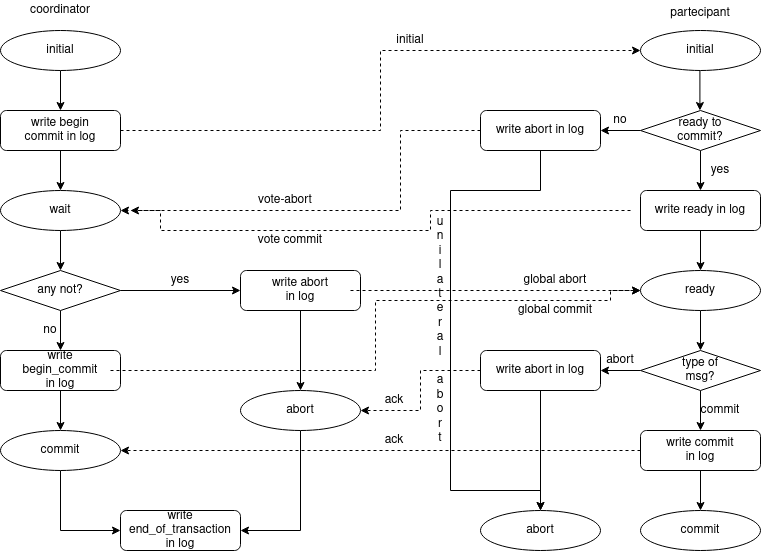
\includegraphics[scale = 0.5]{img/2pc.png}
  \caption{Diagramma del protocollo 2PC, dove negli ovali abbiamo le\emph{
      decisioni} e nei rettangoli le \emph{azioni sui log}. Entrambi i tipi di
    frecce indicano un \emph{messaggio}. La prima fase è fino alle decisioni
    globali incluse.}
  \label{fig:2pc}
\end{figure}
Ai log del TM vengono aggiunti ulteriori dettagli:
\begin{itemize}
  \item \textbf{prepare record} (in figura \ref{fig:2pc} \textit{begin\_commit})
  che contiene l'identità (nodi e transazioni) di tutti i RMs
  \item \textbf{global commit} o \textbf{global abort} che descrive la decisione
  globale. La decisione del TM diventa esecutiva quando scrive nel proprio log
  \textbf{global commit} o \textbf{global abort} 
  \item \textbf{complete record} (in figura \ref{fig:2pc}
  \textit{begin\_of\_transaction}), che viene scritto alla fine del protocollo
\end{itemize}
Al log dei RMs vengono aggiunti ulteriori dettagli:
\begin{itemize}
  \item \textbf{ready record}, per segnalare la disponibilità irrevocabile a
  partecipare alla fase di commit. Si hanno diverse politiche sul
  \textbf{protocollo 2PL} (\textit{recoverable, 2PL, ACR, strict 2PL}). Inoltre
  questo log contiene l'indicazione del TM e i records (come nel caso
  centralizzato), ovvero \textit{begin, insert, delete, update, commit}
  \item \textbf{not ready record} (in figura \ref{fig:2pc} \textit{abort}) per
  segnalare l'indisponibilità del RM al commit
\end{itemize}
In entrambe le fasi del 2PC possono avvenire guasti e in entrambe tutte le
componenti devono poter decidere in base al loro stato. Viene quindi introdotto
l'uso di \textbf{timers}, stabilendo un \textbf{timeout} entro il quale il TM
aspetta una risposta (in entrambe le fasi, anche se nella prima è più
importante). Se il timeout viene superato si lancia un \textit{abort}. Vediamo
distinte le due fasi
\begin{enumerate}
  \item il TM scrive \textit{prepare} nel suo log e invia \textit{prepare} ai
  RMs, fissando un timeout massimo per le riposte. Gli RMs \textit{recoverable},
  ovvero pronti al \textit{commit}, scrivono \textit{ready} nel loro log e
  inviano \textit{ready} al TM. Gli RMs non \textit{recoverable},
  ovvero non pronti al \textit{commit} a causa di un deadlock, scrivono
  \textit{not-ready} nel loro log e terminano il protocollo, con un \textit{log
    unilaterale}. Il TM, come detto scrive nel suo log  \textbf{global commit} o
  il \textbf{global abort}, il secondo nel caso in cui ci sia anche solo un
  \textit{not-ready} o che scatti il timeout (assumendo che i nodi che non hanno
  risposto siano in \textit{failure}).
  \item il TM trasmette la decisione globale e fissa un secondo
  \textit{timeout}. Gli RMs \textit{ready} agiscono di conseguenza scrivendo
  \textit{commit} o \textit{abort} nei loro log e inviando un \textit{ack} al
  TM. Solo dopo effettuano in locale \textit{commit} o \textit{abort}. Il TM
  raccoglie gli \textit{ack} e, in assenza di qualche risposta, fissa un nuovo
  \textit{timeout} ripetendo la trasmissione per gli RMs problematici. Questo
  fino a che non avrà ricevuto da tutti un \textit{ack} e in quel momento scrive
  \textit{complete} nel suo log
\end{enumerate}
Abbiamo quindi appena visto un \textbf{paradigma centralizzato} ``master-salve''
dove i vari RMs non comunicano tra loro. Il TM è quindi il collo di bottiglia''.
Si hanno altri paradigmi:
\begin{itemize}
  \item \textbf{lineare}, dove gli RMs hanno un ordine prestabilito e comunicano
  sempre secondo un ordine prestabilito. Il TM
  è solo il primo di tale ordine. Questo paradigma è utile per reti senza
  possibilità di \textit{broadcast}
  \item \textbf{distribuito}. In questo caso nella prima fase il TM comunica coi
  vari RMs, che però rispondono a tutti. I vari RMs decidono in base alle
  informazioni ricevute dagli altri RMs (comunicano tra loro in
  \textit{broadcast}) e quindi non è più necessaria la seconda fase di
  \textit{2PC}. Si genera una gran quantità di messaggi tra i vari RMs, avendo
  una situazione ``tra pari'' \textit{Peer-to-Peer}, creando un problema di
  prestazioni, dovendo garantire la comunicazione tra tutti i nodi (anche
  tramite \textit{ack})
\end{itemize}
\subsubsection{2PC in caso di guasto}
In uno stato di guasto, nel caso \textbf{centralizzato}, un RM nello stato
\textit{ready} perde la sua autonomia e attende la decisione del TM. Nel caso di
guasto del TM i vari RMs sono lasciati in \textit{stato di incertezza} e le
risorse allocate alla transazione restano bloccate.
\begin{definizione}
  Definiamo \textbf{finestra di incertezza} come la finestra temporale fra la
  scrittura di ready nel log dei RMs e la scrittura di \emph{commit} o
  \emph{abort}. Questo intervallo è ridotto al minimo da \textbf{2PC}.
\end{definizione}
Durante la finestra di incertezza tutte le risorse acquisite tramite meccanismi
di \textit{lock} restano bloccate e, in caso di guasto durante la
\textit{finestra di incertezza}, TM e RMs usano i \textbf{protocolli di
  recovery}.\\
Si possono avere diversi guasti:
\begin{itemize}
  \item \textbf{guasti di componenti}, ovvero guasti al TM o ai RMs.
  \item \textbf{perdita di messaggi o partizionamento della rete}
\end{itemize}
\paragraph{Guasti di componenti}
In questo caso devono essere usati protocolli con due compiti:
\begin{enumerate}
  \item assicurare la terminazione delle procedure. Sono i \textbf{protocolli di
  terminazione}
\item assicurare il ripristino. Sono i \textbf{protocolli di recovery}
\end{enumerate}
\textbf{In entrambi i casi questi protocolli funzionano sia che il guasto
  interessi un solo componente che più di uno}.\\
Partiamo dal caso in cui cada un RM. Può cadere prima di iniziare il protocollo,
non rispondendo al \textit{prepare} e portando all'\textit{abort}. Può cadere
dopo il \textit{ready\_to\_commit} e se quando si riprende vede nei log lo stato
\textit{ready} si mette in \textit{wait} non sapendo bene come fare (nel caso di
\textit{abort} semplicemente chiuderà il protocollo). Il TM
provvederà a inviare a tale RM \textit{commit} o \textit{abort}. Non si hanno
quindi problemi al protocollo, o si va diretti all'\textit{abort} o si
aspetta. Il TM capisce che un RM è caduto grazie al \textit{timeout}.\\
Più complesso è il caso in cui cada il TM. Se cade prima di ricevere le risposte
al \textit{prepare}, quando si sarà ripreso, guarderà lo stato delle risposte al
\textit{prepare} ricevute, altrimenti si avrà un \textit{abort unilaterale}. \\
Vengono introdotti gli \textbf{algoritmi bizantini} nel caso in cui il TM cada e
il RMs debbano decidere insieme cosa fare. Per decidere serve visibilità.\\
Quindi, ricapitolando per le cadute del TM:
\begin{itemize}
  \item cade quanto l'ultimo record del log è \textit{prepare}, magari bloccando
  alcuni RMs. In tal caso si hanno 2 opzioni di recovery:
  \begin{enumerate}
    \item decidere \textit{global abort}, e procedere con la seconda fase di 2PC
    \item ripetere la prima fase, sperando di giungere a un \textit{global
      commit}, richiedendo nuovamente lo stato dei RM
  \end{enumerate}
  \item cade quanto l'ultimo record del log è \textit{global-commit} o
  \textit{global-abort} il TM deve ripete la seconda fase in quanto alcuni RMs
  potrebbero essere bloccati o comunque ignari della decisione presa prima della
  caduta
  \item l’ultimo record nel log è una \textit{complete}, in tal caso non si
  hanno problemi
\end{itemize}
Ricapitoliamo anche le cadute dell'RM:
\begin{itemize}
  \item l'ultimo record nei log è di \textit{azione}, \textit{abort} o
  \textit{commit}, come nel caso centralizzato e in tal caso di procede con un
  \textbf{warm restart}:
  \begin{itemize}
    \item nel caso di \textit{abort} o \textit{azione} si procede con
    l'\textit{undo} dell'operazione
    \item nel caso di \textit{commit} di effettua nuovamente la transazione
  \end{itemize}
  \item l'ultimo record nei log è \textit{ready} e in tal caso l'RM si blocca
  non conoscendo la decisione del TM e si inseriscono, durante \textit{warm
    restart}, nel \textit{ready set} le transazioni dubbie. Si hanno quindi due
  alternative:
  \begin{enumerate}
    \item \textbf{remote recovery}, ovvero l'RM chiede al TM cosa è accaduto
    \item il TM riesegue la seconda fase del protocollo
  \end{enumerate}
\end{itemize}
\paragraph{Perdita di messaggi e partizionamento della rete}
In questo caso il TM non riesce a distinguere tra perdita di messaggi
\textit{prepare} o \textit{ready} nella prima fase e procede, scattando i
\textit{timeout}, con un \textbf{global abort}. \\
Durante la seconda fase la non distinzione tra perdita di \textit{ack} o di
decisioni dei gli RM porta alla ripetizione della seconda fase dopo il
\textit{timeout}.\\
% Un partizionamento della rete non causa problemi ulteriori, dato che una
% transazione può avere successo solo se il TM e tutti i RM appartengono alla
% stessa partizione.
Se durante lo svolgimento del protocollo 2pc si partiziona la rete avendo due
sottoreti una con TM e RM1 che e la seconda sottorete con RM2, RM3. In questo
caso il TM continua a mandare il messaggio della global decision a RM2 RM3 dopo
lo scadere del timeout. Si concluderà comunque, con alte probabilità, con un
\textit{abort} da parte del TM.
\subsubsection{Ottimizzazioni di 2PC}
2PC può essere ottimizzato per:
\begin{itemize}
  \item ridurre il numero di messaggi tra TM e RMs
  \item ridurre le scritture nei log
\end{itemize}
Si hanno due tipi di ottimizzazione:
\begin{enumerate}
  \item \textbf{ottimizzazione read-only}, quando un RM sa che se la propria
  transazione è \textit{read-only} allora non influenza l'esito finale della
  transazione. Al \textit{prepare} risponde \textit{read-only} e termina il
  protocollo. Il TM ignora i partecipanti \textit{read-only} dalla seconda fase
  e, qualora si sapesse a priori, possono anche essere direttamente esclusi dal
  protocollo
  \item \textbf{ottimizzazione presumed abort} che si basa sulla regola
  ``scordarsi gli \textit{abort} e ricordasi i \textit{commit}''. In questo caso
  il TM abbandona la transazione dopo la decisione di abort senza scrivere
  \textit{global abort} nel log e senza aspettare risposta dai vari RMs. Se il
  TM riceve richiesta di un \textit{remote recovery} il TM decide per il
  \textit{global abort}. Non sarà più necessario quindi scriver e\textit{global
    abort} o \textit{prepare} nei log ma solo \textit{global commit, ready} e
  \textit{commit}
\end{enumerate}
\subsubsection{Protocollo X/Open}
Il protocollo 2PC è stato adottato nel protocollo \textbf{X/Open DTP
  (\textit{Distributed Transaction Processing})}, che è un 
consorzio di vendors che vogliono rendere portabile lo standard dell'ambiente
UNIX. In questo protocollo si ha il \textit{TX interface} per la comunicazione
tra il TM e l'applicazione e si ha l'\textit{XA interface} per la comunicazione
tra TM e RMs. Ogni vendor ha la sua implementazione del modello.
\section{Repliche}
Parliamo ora delle tecnologie per la \textbf{replicazione di dati}.\\
Tra le principali soluzioni architetturale troviamo \textbf{IBM replication
  technologies} e \textbf{Microsoft SQL Server replication technologies}
(\textit{i dettagli delle implementazioni non saranno oggetto d'esame}).\\
\begin{definizione}
  La \textbf{replica} è il processo di cerare e mantenere istanze dello stesso
  db allineate tra loro, consentendo la condivisione di dati ma anche
  comportando cambiamenti architetturali. Si ha che le eventuali modifiche
  devono essere viste da tutti i nodi.
\end{definizione}
\begin{definizione}
  Definiamo \textbf{sincronizzazione} è il processo che m i consente di
  \textit{allineare} le copie, prima o poi.
\end{definizione}
In base all'ultima definizione si capisce che spesso le copie non sono
aggiornate istantaneamente. Si ha quindi la \textbf{replica sincrona} o la
\textbf{replica asincrona} (non avendo allineamento \textit{realtime}). IBM
preferisce un approccio \textit{based and mode based} mentre Microsoft uno
basato su \textit{snapshot, transactional \textnormal{e} merge}.\\
Vediamo le differenze tra le due repliche:
\begin{itemize}
  \item le \textbf{repliche sincrone} cercano di far si che tutte le repliche
  vengano aggiornate contemporaneamente (ad esempio si ha il protocollo
  ROWA). Scrivo in modo sincrono su tutti nodi e solo quando tutte le repliche
  confermano la scrittura avanzo con le transazioni (che fallisce se ho nodi non
  disponibili). Nelle repliche sincrone si necessitano molti scambi di messaggi.
  Di fatto si obbliga due o più \textit{storage} ad aggiornarsi e a fare
  \textit{rollback} in caso di fallimento. Si hanno quindi alte disponibilità,
  un auto \textit{fail-over} (bloccando la transazioni in caso di guasti sui
  nodi) e un \textit{data loss} minimo. Le repliche sincrone vengono soprattutto
  usate nei \textit{disaster recovery}, ovvero in situazioni \textit{mission
    critical} (ad esempio sistemi bancari dove i db di backup, almeno 3, devono
  stare a centinaia di kilometri di distanza, in zone sismiche tra loro
  diverse). Gli svantaggi delle repliche sincrone sono la necessità di una rete
  valida, si hanno problemi di scalabilità, di costi e minor flessibilità
  \item nelle \textbf{repliche asincrone} prima si aggiorna il db
  \textit{target} e poi le repliche (normalmente dopo pochi secondi ma anche
  dopo giorni). Si hanno evidenti vantaggi di costo, scalabilità e flessibilità
  (perché in caso di problema lavoro in primis sul db principale)
  ma a rischio di \textit{data loss} (nell'intervallo di tempo tra la scrittura
  del db principale e delle repliche). Normalmente si usano soluzioni asincrone
  per accessi online e la loro efficienza, per bilanciamento del calcolo
  etc$\ldots$ 
\end{itemize}
\textit{In caso di perdita di dati bisogna analizzare i singoli contratti per
  capire legalmente come rispondere di dati che non verranno recuperati
  probabilmente.}\\
Ci sono vari contesti in cui pensare alla replica dei dati:
\begin{itemize}
  \item condivisione di dati da utenti tra loro scollegati. Un esempio è una
  copia su un portatile con una replica usata da un commerciale. Si possono
  avere conflitti nel momento in cui più utenti con db replicati lavorano
  offline. Si ha il \textit{merge conflict}
  \item \textit{data consolidation}, ovvero quando un'azienda vuole tenere più
  copie dei dati in vari punti e alla fine bisogna riportare i dati a livello
  centrale a cadenza periodica. Può servire per fare data warehousing o anche
  solo semplicemente per monitorare le vendite delle varie filiali o per
  aggiornare il catalogo
  \item \textit{data distribution} che è il caso degli \textit{e-commerce}. È un
  caso tipicamente \textit{mission-critical} e bisogna aumentare l'accesso ai
  dati e si ha una costante sincronizzazione realtime bidirezionale per evitare
  problemi. Un altro caso è la distribuzione tra diversi uffici, dove le
  repliche locali hanno magari dati non presenti nel db globale
  \item prestazioni, accesso efficiente, \textit{load balancing} e accesso
  offline. Se non si hanno necessità di update immediati (tipo un sito vetrina)
  allora la replica garantisce la disponibilità e l'accessibilità a basso
  costo. Con il load balancing scarico gli utenti su diverse macchine replicate,
  in primis per le molte realtà di sola lettura o comunque con pochissime
  scritture (un esempio può anche essere un social network dove anche eventuali
  ritardi di qualche secondo non sono problematici). Per la disponibilità
  bisogna fare un forte testing dell'intera architettura, se cade un server
  bisogna puntare ad una replica e bisogna essere sicuri e spesso i costi sono
  troppo alti (\textit{RIVEDERE QUESTA PARTE})
  \item separazione tra \textit{data entry \textnormal{e} reporting}, se si
  usa lo stesso server per entrambi i compiti (che in pratica sono scrittura
  costante e lettura costante) può essere utile separare in due server. Si
  evitano così i rallentamenti dati dai \textit{lock}. Bisogna studiare i tempi
  di sincronizzazione
  \item coesistenza di applicazioni, questo è un caso particolare. Qualora
  sia necessario cambiare applicazione devo, eventualmente, cambiare anche i
  sistemi. Bisogna quindi travasare i dati vecchi e durante il trasferimento
  bisogna comunque mantenere funzionanti le applicazioni. Quindi bisogna far
  coesistere i due database durante il trasferimento (facendo il travaso di
  notte bloccando le transazioni). I costi sono incredibili e si può avere anche
  coesistenza delle applicazioni e non solo dei dati, con migrazioni parziali
  (magari per area geografica) etc$\ldots$ questo comporta che magari due
  filiali devono collaborare con due applicazioni e due db diversi
\end{itemize}
Ci sono anche casi in cui non si dovrebbe replicare:
\begin{itemize}
  \item quando ci sono frequenti update su più copie, portando le copie a
  possibili conflitti che devono essere scoperti e gestiti ``manualmente'' 
  \item quando la consistenza è \textit{critical} magari in contesti di
  trasferimento di fondi etc$\ldots$. In questo caso solitamente si impone un
  protocollo ROWA (con transazioni \textit{ACID compliant}), riducendo le
  prestazioni per avere l'autorizzazione dei \textit{commit} da parte delle
  repliche 
\end{itemize}
Ma spesso bisogna comunque replicare ``scegliendo il male minore'' (ad esempio
nelle banche) e bisogna quindi analizzare il singolo caso, anche in base al
budget. Inoltre non bastano le tecnologie serve un'ottima organizzazione.\\ 
Concludendo si ha che i benefici della replica sono:
\begin{itemize}
  \item disponibilità
  \item affidabilità
  \item prestazioni
  \item riduzione di carico
  \item lavoro offline
  \item supporto a molti utenti
\end{itemize}
Distinguiamo anche delle classi di tipologie di replica:
\begin{itemize}
  \item \textbf{data distribution}, di tipo \textit{1:many}, con un
  \textit{source} che distribuisce, in modo sincrono o asincrono, le varie copie
  passive ai \textit{target}
  \item \textbf{Peer-to-Peer}, dove i vari nodi sono interconnessi e si
  aggiornano tra di loro. Si usa un approccio ROWA
  \item \textbf{data consolidation}, di tipo \textit{many:1}, dove ho più
  \textit{source} che aggiornano un \textit{target} a livello centrale
  \item \textbf{bi-directional} (per il \textit{conflict detention resolution}),
  dove una copia primaria e uno secondaria 
  possono leggere e scrivere a vicenda tra loro (è quindi una versione
  semplificata del \textit{Peer-to-Peer} con due Peer)
  \item \textbf{multi-Tier staging}, in cui si hanno meccanismi intermedi tra
  \textit{source} e \textit{target} con ``aree di deposito'' dette aree di
  \textit{staging}
\end{itemize}
Per realizzare una replica posso fare in diversi modi:
\begin{itemize}
  \item faccio letteralmente il backup del disco con una persona che stacca il
  disco dal server e lo copia, riattaccando infine copia e disco originale
  \item posso prima fare il backup attaccando un altro disco e poi mettere nella
  nuova macchina il disco copia
  \item posso fare una \textit{replica incrementale}, ovvero faccio un
  \textit{full backup} e sposto solo il file di \textit{log} delle transazioni
  nel nuovo server, rieseguendo quanto fatto (essendo contenuto nel
  \textit{log}). Quindi prima faccio un \textit{full
    backup} e poi un \textit{backup \textnormal{del} log}, questo per ogni
  replica. Un'alternativa è l'\textbf{event publish}.
  Un \textbf{event publish} è una replica senza \textit{apply} e
  leggo i file di log. Analizzando gli eventi tramite particolari meccanismi
  riscrivo quindi sull'architettura target. Da un \textit{publisher} si passa ad
  un \textit{distributor} e infine ai \textit{subscriber}
  % MANCA PARTE DB2
\end{itemize}
\textbf{Sulle slide \textit{repliche} si ha un approfondimento delle
  architetture IBM e Microsoft opzionali per il corso}.\\
\begin{shaded}
  Un \textbf{db parallelo} è studiato per le prestazioni. Si ha accesso
  parallelo ai dati, parallelismo \textit{intra-query} (stessa query su
  frammenti diversi), parallelismo \textit{inter-query} (tante query diverse) e
  sono fatti da elementi hardware posti vicini tra loro.\\
  Parliamo di \textbf{persistenza dei dati}. Bisogna garantire la durabilità dei
  dati, bisogna quindi usare un db. Si hanno anche problemi per creare oggetti
  persistenti a partire da un linguaggio OOP, si ha il cosiddetto
  l'\textbf{object-relational paradigm mismatch}. Si separa quindi l'aspetto OOP
  e l'aspetto relazionale per risolvere il problema per poi ``mappare'' l'uno
  nell'altro, tramite i \textbf{data mapper}. Si hanno operazioni \textbf{CRUD}:
  \begin{itemize}
    \item Create
    \item Read
    \item Update
    \item Delete
  \end{itemize}
  Si ha quindi il cosiddetto \textbf{Object–relational mapping}, ovvero questa
  tecnica di mapping. Si hanno vari framework che lo implementano.\\
  Storicamente si è provato a fare db ad oggetti ma con scarsi risultati.
\end{shaded}
\section{Prima esercitazione}
\begin{esercizio}
  Si consideri un db con le seguenti relazioni (e quindi tabelle):
  \begin{itemize}
    \item PRODUCTION (\underline{SerialNumber}, PartType, Model, Quantity,
    Machine) 
    \item PICKUP (\underline{SerialNumber}, \underline{Lot}, \textbf{Client,
      SalesPerson},  Amount) 
    \item CLIENT (\underline{Name}, City, Address)
    \item SALESPERSON (\underline{Name}, City, Address)
  \end{itemize}
  \textit{(con sottolineate le chiavi primarie e in grassetto le chiavi di
    integrità referenziale)}\\
  
  e ci poniamo l'obiettivo di partizionare il db secondo determinate
  specifiche.\\
  Si assume che si abbiano le seguenti specifiche organizzative:
  \begin{itemize}
    \item si hanno 4 centri di produzione (\textit{Dublino, San Jose, Zurigo
      \textnormal{e} Taiwan}, ciascuno responsabile, rispettivamente, di
    \textit{cpu, keyboard, screen \textnormal{e} cable}) e 3 centri di vendita
    (\textit{San Jose, Zurigo  \textnormal{e} Taiwan})
    \item le vendite sono distribuite secondo le località geografiche, i clienti
    a Zurigo sono serviti solo dai venditori di Zurigo etc$\ldots$. SI ha però
    che i venditori di  Zurigo servono anche Dublino
    \item ogni area geografica ha il proprio db (avremo quindi 4 db)
  \end{itemize}
  Vogliamo studiare una \textbf{frammentazione orizzontale} delle 4 tabelle.\\
  Ricordiamo quindi che abbiamo 4 centri di produzione (ciascuno responsabile di
  un prodotto e con un db ciascuno) e 3 punti di vendita.\\
  Partiamo con la frammentazione della relazione \textnormal{PRODUCTION},
  ottenendo 4 tabelle, una per componente prodotto, ottenendo (con $\sigma$
  abbiamo l'operazione di selezione nell'algebra relazionale):
  \begin{itemize}
    \item $PRODUCTION_1=\sigma_{partType=cpu}(PRODUCTION)$
    \item $PRODUCTION_2=\sigma_{partType=keyboard}(PRODUCTION)$
    \item $PRODUCTION_3=\sigma_{partType=screen}(PRODUCTION)$
    \item $PRODUCTION_4=\sigma_{partType=cable}(PRODUCTION)$    
  \end{itemize}
  Passiamo alla relazione \textnormal{PICKUP}. Anche in questo caso si frammenta
  per il prodotto facendo il join con la tabella
  \textnormal{PRODUCTION}(ricordando che $\pi$ è l'operazione di proiezione/join 
  nell'algebra relazionale). Per comodità indichiamo tutti gli attributi di
  \textnormal{PICKUP} con $pick$, avendo quindi:
  \[pick=SerialNumber, Lot, Client, SalesPerson, Amount\]
  indico anche con $SN$ $SerialNumber$
  \begin{itemize}
    \item \scriptsize{$PICKUP_1=\pi_{pick}(\sigma_{partType=cpu}(PICKUP\,\, SN
      =SN(PRODUCTION)))$}   
    \item \scriptsize{$PICKUP_2=\pi_{pick}(\sigma_{partType=keyboard}(PICKUP\,\, SN
      =SN(PRODUCTION)))$}   
    \item \scriptsize{$PICKUP_3=\pi_{pick}(\sigma_{partType=screen}(PICKUP\,\, SN
      =SN(PRODUCTION)))$}  
    \item \scriptsize{$PICKUP_4=\pi_{pick}(\sigma_{partType=cable}(PICKUP\,\, SN
     =SN(PRODUCTION)))$}  
 \end{itemize}
 Prendo quindi una proiezione di tutti gli elementi di \textit{PICKUP} separando
 nei vari \textit{PICKUP} in base al prodotto.\\
 Passo a alle tabelle \textnormal{SALESPERSON}. Abbiamo 3
 punti di vendita, quindi, circa come per \textnormal{PRODUCTION}, frammento in
 base alle città di vendita:
 \begin{itemize}
   \item $SALESPERSON_1=\sigma_{City="San Jose"}(SALESPERSON)$
   \item $SALESPERSON_2=\sigma_{City="Zurigo"}(SALESPERSON)$
   \item $SALESPERSON_3=\sigma_{City="Taiwan"}(SALESPERSON)$
 \end{itemize}
 Manca solamente \textnormal{CLIENT}. Anche in questo caso divido in base alle
 città, ricordando che Zurigo e Dublino sono clienti entrambi di Zurigo:
  \begin{itemize}
   \item $CLIENT_1=\sigma_{City="San Jose"}(CLIENT)$
   \item $CLIENT_2=\sigma_{City="Zurigo"\mbox{ or }City="Dublino"}(CLIENT)$
   \item $CLIENT_3=\sigma_{City="Taiwan"}(CLIENT)$
 \end{itemize}
 Abbiamo finito la frammentazione e quindi dobbiamo solo distribuire tali
 tabelle: 
 \begin{itemize}
   \item le quattro tabelle con indice 1 andranno a San Jose, in
   \texttt{company.sanjose.com}
   \item le quattro tabelle con indice 2 andranno a Zurigo, in
   \texttt{company.zurigo.com} 
   \item le quattro tabelle con indice 3 andranno a Taiwan, in
   \texttt{company.taiwan.com} 
   \item le due tabelle con indice 4 andranno a Dublino (che quindi avrà solo
   parte di \textnormal{PRODUCTION} e parte di \textnormal{PICKUP} in quanto a
   Dublino non si ha un punto vendita), in \texttt{company.dublino.com}
 \end{itemize}
\end{esercizio}
\begin{esercizio}
  Vediamo un esercizio in merito alla trasparenza, che ricordiamo essere a tre
  livelli:
  \begin{enumerate}
    \item di frammentazione
    \item di replicazione/allocazione
    \item di linguaggio
  \end{enumerate}
  Si chiede di fare delle interrogazioni, tenendo conto dei livelli di
  trasparenza, sul db costruito nell'esercizio precedente.\\
  La prima query ci chiede di determinare la quantità dei prodotti che hanno
  valore ``77y6878'' (abbiamo quindi a che fare con la trasparenza di
  frammentazione, infatti interroghiamo come se avessimo a che fare con un solo
  db): 
  \begin{minted}{sql}
    Procedure Query1(:Quan):
     Select Quantity in :Quan
     From PRODUCTION
     Where SerialNumber="77y6878"
    End Procedure
  \end{minted}
  (con \texttt{:Quan} indichiamo il nome della tabella).\\
  Vediamo ora come fare nel caso di trasparenza di allocazione, quindi si sa di
  avere a che fare con un db distribuito. La query quindi si ``sposterà'' alla
  ricerca del giusto frammento:
  \begin{minted}{sql}
    Procedure Query2(:Quan):
     Select Quantity in :Quan
     From PRODUCTION_1
     Where SerialNumber="77y6878"
     
     if :empty then
     Select Quantity in :Quan
     From PRODUCTION_2
     Where SerialNumber="77y6878"
     
     if :empty then
     Select Quantity in :Quan
     From PRODUCTION_3
     Where SerialNumber="77y6878"
     
     if :empty then
     Select Quantity in :Quan
     From PRODUCTION_4
     Where SerialNumber="77y6878"
    End Procedure
  \end{minted}
  Vediamo ora come funziona per la trasparenza di linguaggio. In tal caso
  dobbiamo considerare sia le frammentazioni che i vari indirizzi di
  allocazione, ovvero i \texttt{company.città.com}:
  \begin{minted}{sql}
    Procedure Query3(:Quan):
     Select Quantity in :Quan
     From PRODUCTION_1@company.sanjose.com
     Where SerialNumber="77y6878"
     
     if :empty then
     Select Quantity in :Quan
     From PRODUCTION_2@company.zurigo.com
     Where SerialNumber="77y6878"
     
     if :empty then
     Select Quantity in :Quan
     From PRODUCTION_3@company.taiwan.com
     Where SerialNumber="77y6878"
     
     if :empty then
     Select Quantity in :Quan
     From PRODUCTION_4@company.dublino.com
     Where SerialNumber="77y6878"
    End Procedure
  \end{minted}
  \textit{Nelle slide usa \texttt{union} al posto di \texttt{if :empty then}}.
\end{esercizio}
\begin{esercizio}
  Sempre sul db del primo esercizio effettuiamo la seguente query:
  \textit{determinare le macchine che utilizzano come componente ``keyboard'' e
    sono vendute al cliente ``Brown''}.\\
  Per praticità vediamo solo la trasparenza di frammentazione e quella di
  allocazione.\\
  Partiamo con la trasparenza di frammentazione:
  \begin{minted}{sql}
    Procedure Query1(:Machine)
     Select Machine in :Machine
     From PRODUCTION join PICKUP on
     PRODUCTION.SerialNumber=PICKUP.SerialNumber
     Where PartType = "keyboard" AND Client="Brown"
    End Procedure
  \end{minted}
  Vediamo il caso di trasparenza di allocazione (e sappiamo che ``keyboard'' è
  solo in $PRODUCTION_2$ quindi interroghiamo un solo frammento e senza chiedere
  la specifica del $partType$):
  \begin{minted}{sql}
    Procedure Query2(:Machine)
     Select Machine in :Machine
     From PRODUCTION_2 join PICKUP on
     PRODUCTION_2.SerialNumber=PICKUP_2.SerialNumber
     Where Client="Brown"
    End Procedure
  \end{minted}
  Se avessimo voluto fare anche la trasparenza di linguaggio non sarebbe
  cambiato nulla dato che $PRODUCTION_2$ è solo a Zurigo.
\end{esercizio}
\begin{esercizio}
  Sempre sul db del primo esercizio effettuiamo il cambiamento di indirizzo del
  cliente ``Brown'' che si sposta da ``27 Church St.'', Dublino, a ``43 Park Hoi
  St.'', Taiwan. Abbiamo quindi un cambio di allocazione nel db.\\
  Partiamo con la trasparenza di frammentazione:
  \begin{minted}{sql}
    Procedure Update1
     Update Client
     Set Address  = "43 Park Hoi St.", City="Taiwan"
     Where Name="Brown"
    End Procedure
  \end{minted}
  La cosa si complica nel caso di trasparenza di allocazione, tenendo conto
  delle due città e dei loro db:
  \begin{minted}{sql}
    Procedure Update2
     Delete CLIENT_2
     Where Name="Brown"
     
     Insert into CLIENT_3 (Name, Address, City)
     values ("Brown", "43 Park Hoi St.", "Taiwan")
    End Procedure
  \end{minted}
  Se avessimo voluto fare anche la trasparenza di linguaggio non sarebbe
  cambiato nulla poiché le frammentazioni sono in locazioni diverse
\end{esercizio}
\begin{esercizio}
  Sempre sul db del primo esercizio effettuiamo la seguente query:\\
  \textit{calcolare la somma di tutti gli ordini ricevuti a SanJose, Zurigo e
    Taiwan}.\\
  Partiamo con la trasparenza di frammentazione:
  \begin{minted}{sql}
    Procedure Query1
     Select City, sum(Amount)
     From PICKUP join SALESPERSON on
     SalesPerson = Name
     Groub by city
    End Procedure
  \end{minted}
  Passiamo alla trasparenza di allocazione. Mi serviranno tutti i frammenti di
  \texttt{SALESPERSON}. Inoltre devo considerare i vari \texttt{PICKUP}, tutti e
  quattro per il discorso delle vendite su Dublino:
  \begin{minted}{sql}
    Procedure Query2
     Create view PICKUP as
     PICKUP_1 union PICKUP_2 union PICKUP_3 union PICKUP_4
     
     Select City, sum(Amount)
     From SALESPERSON_1 join PICKUP on
     SalesPerson=Name
     union
     From SALESPERSON_2 join PICKUP on
     SalesPerson=Name
     union
     From SALESPERSON_3 join PICKUP on
     SalesPerson=Name
    End Procedure
  \end{minted}
\end{esercizio}
\begin{esercizio}
   Sempre sul db del primo esercizio cerchiamo di massimizzare il parallelismo
   delle inter-query.\\
   Prendiamo la seguente query:
   \textit{estrarre la somma delle quantità di produzione che sono raggruppate
     secondo i tipi e i modelli delle componenti}.\\
   \begin{minted}{sql}
    Procedure Query1
     Select sum(Quantity), Model, PartType
     from PRODUCTION
     Group by (Model, PartType)
    End Procedure
  \end{minted}
  Vogliamo però massimizzare il parallelismo, divido quindi tra le varie
  frammentazioni:
  \begin{minted}{sql}
    Procedure Query1
     Select sum(Quantity), Model, PartType
     from PRODUCTION_1
     Group by (Model, PartType)

     Select sum(Quantity), Model, PartType
     from PRODUCTION_2
     Group by (Model, PartType)

     Select sum(Quantity), Model, PartType
     from PRODUCTION_3
     Group by (Model, PartType)

     Select sum(Quantity), Model, PartType
     from PRODUCTION_4
     Group by (Model, PartType)
    End Procedure
  \end{minted}
  massimizziamo il parallelismo inter-query se si consideriamo che ogni
  partizione ha un DBMS diverso. Volendo potrei dividere la query ancora a
  seconda del modello, evitando il \texttt{group by} (cosa utile nel caso in cui
  si abbia a che fare con un sistema fortemente multicore)
\end{esercizio}
\begin{esercizio}
  Vediamo un esempio di db replicato che può produrre inconsistenza.\\
  Prendiamo l'esempio del db prodotto nel primo esercizio. Supponiamo che ogni
  frammento di \textnormal{PRODUCTION} sia allocato a tutti i DBMS. Però ogni
  DBMS utilizza un frammento e trasmette i cambiamenti del frammento agli altri
  DBMS, permettendo di avere copie del db. In caso di fallimento di un DBMS il
  db sarebbe comunque accessibile dagli altri sistemi e non so avrebbe problemi
  con le query, avendo che il fallimento è trasparente sia ai client che al db
  stesso. Purtroppo quando si ha un fallimento si può generare un
  partizionamento di rete e questo può comportare delle inconsistenze. Se, per
  esempio, due transazioni tolgono 800 ad una certa quantità la seconda in
  ordine temporale fallirà ma se avvengono in due DBMS non connessi non
  falliranno, producendo inconsistenza.
\end{esercizio}
\begin{esercizio}
  Data una replicazione simmetrica dire quando produce inconsistenza.
  Un esempio è un db senza il \textit{concurrency control} e quindi due
  transazioni come quelle dell'esercizio precedente possono causare
  inconsistenza anche senza fallimento della rete.
\end{esercizio}
\chapter{Blockchains}
\textbf{\textit{Questa lezione è stata tenuta dal prof. Leporati}}.\\
\textbf{Nonostante qualche ambiguità ed errore di scrittura, nel capitolo si
  userà il termine ``nodo'' 
  quando si parla di rete P2P e il termine ``blocco'' quando ci si riferisce ai
  blocchi interni alla blockchain.}
\begin{definizione}
  Una \textbf{blockchain}, in poche parole, è un registro pubblico, condiviso e
  decentralizzato che memorizza la proprietà di beni digitali. 
\end{definizione}
È quindi un registro in cui vengono memorizzate informazioni relative alla
proprietà di qualcosa che può essere rappresentato tramite sequenze di bit
(quindi qualcosa di digitale come i \textit{bitcoin} o altre criptovalute).\\
Vengono memorizzate anche le \textbf{transazioni}, ovvero i cambi di
proprietà.\\
Essendo pubblico tutti possono vedere cosa è stato registrato e in particolare
``chi possiede cosa'' e la storia di una certa proprietà.\\
Questo registro è condiviso in quanto gestito da più persone ed è
decentralizzato in quanto non esiste un nucleo che abbia di poteri da
amministratore rispetto agli altri, tutti sono allo stesso livello.
\\
Questo registro è organizzato in blocchi. Si ha un primo blocco detto
\textbf{genesis block} che da il via a tutto. Si hanno poi altri blocchi, in
nero, collegati a questo e che formano una catena. Un blocco si lega al
successivo tramite particolari funzioni crittografiche, dette \textbf{funzioni
  di hash crittografico}. Nel dettaglio il collegamento tra un blocco e il
successivo è dato dal fatto che il valore di hash del blocco è contenuta
all'interno del blocco successivo, facendo in modo che si estremamente
difficile alterare il contenuto di un blocco, ovvero diverse transazioni, che
sono organizzate secondo una precisa struttura dati che consente di verificare
la validità in modo veloce ed efficiente. Per ogni blocco si calcola quindi
l'hash e lo si salva nel blocco successivo. Per modificare una transazione
quindi dovrei calcolare l'hash e dovrei fare il check con il blocco
successivo. Quindi tutti possono verificare la validità della
blockchain. Modificare i dati in modo tale da ottenere lo stesso hash però è
davvero difficile.\\
\begin{figure}
  \centering
  
  \psscalebox{1.3 1.3} % Change this value to rescale the drawing.
  {
    \begin{pspicture}(0,-1.0)(6.8,1.0)
      \definecolor{colour0}{rgb}{0.08235294,0.61960787,0.22352941}
      \definecolor{colour1}{rgb}{0.9529412,0.25882354,0.25882354}
      \psframe[linecolor=colour0, linewidth=0.02, dimen=outer,
      framearc=0.35](0.4,0.6)(0.0,0.2)
      \psframe[linecolor=colour1, linewidth=0.02, dimen=outer,
      framearc=0.35](2.0,1.0)(1.6,0.6)
      \psframe[linecolor=black, linewidth=0.02, dimen=outer,
      framearc=0.35](2.0,0.2)(1.6,-0.2)
      \psframe[linecolor=black, linewidth=0.02, dimen=outer,
      framearc=0.35](1.2,0.6)(0.8,0.2)
      \psframe[linecolor=black, linewidth=0.02, dimen=outer,
      framearc=0.35](2.8,0.2)(2.4,-0.2)
      \psframe[linecolor=black, linewidth=0.02, dimen=outer,
      framearc=0.35](3.6,0.2)(3.2,-0.2)
      \psframe[linecolor=black, linewidth=0.02, dimen=outer,
      framearc=0.35](4.4,0.2)(4.0,-0.2)
      \psframe[linecolor=black, linewidth=0.02, dimen=outer,
      framearc=0.35](5.2,0.6)(4.8,0.2)
      \psframe[linecolor=black, linewidth=0.02, dimen=outer,
      framearc=0.35](6.0,0.6)(5.6,0.2)
      \psframe[linecolor=black, linewidth=0.02, dimen=outer,
      framearc=0.35](6.8,0.6)(6.4,0.2)
      \psline[linecolor=black, linewidth=0.02](0.4,0.4)(0.8,0.4)
      \psline[linecolor=black, linewidth=0.02](1.1627907,0.3860465)
      (1.6279069,0.8511628)
      \psline[linecolor=black, linewidth=0.02](1.1627907,0.3860465)
      (1.6279069,0.013953488)
      \psline[linecolor=black, linewidth=0.02](2.0,0.013953488)
      (2.372093,0.013953488)
      \psline[linecolor=black, linewidth=0.02](2.7441862,0.013953488)
      (3.2093024,0.013953488)
      \psline[linecolor=black, linewidth=0.02](3.5813954,0.013953488)
      (4.0465117,0.013953488)
      \psline[linecolor=black, linewidth=0.02](4.418605,0.013953488)
      (4.7906976,-0.35813954)
      \psline[linecolor=black, linewidth=0.02](5.162791,-0.35813954)
      (5.627907,-0.35813954)
      \psline[linecolor=black, linewidth=0.02](5.162791,0.3860465)
      (5.627907,0.3860465)
      \psline[linecolor=black, linewidth=0.02](6.0,0.3860465)
      (6.372093,0.3860465)
      \psline[linecolor=black, linewidth=0.02](4.418605,0.013953488)
      (4.7906976,0.3860465)
      \psline[linecolor=black, linewidth=0.02](3.3953488,-0.17209302)
      (3.3953488,-0.6372093)
      \psline[linecolor=black, linewidth=0.02](3.5813954,-0.82325584)
      (4.0465117,-0.82325584)
      \psframe[linecolor=colour1, linewidth=0.02, dimen=outer,
      framearc=0.35](3.6,-0.6)(3.2,-1.0)
      \psframe[linecolor=colour1, linewidth=0.02, dimen=outer,
      framearc=0.35](4.4,-0.6)(4.0,-1.0)
      \psframe[linecolor=colour1, linewidth=0.02, dimen=outer,
      framearc=0.35](5.2,-0.2)(4.8,-0.6)
      \psframe[linecolor=colour1, linewidth=0.02, dimen=outer,
      framearc=0.35](6.0,-0.2)(5.6,-0.6)
    \end{pspicture}
  }
  \caption{Esempio di schema di blockchain. In verde a sinistra troviamo il
    \textbf{genesis block}. In nero i blocchi che formano la catena. In rosso
    abbiamo i nodi \textit{orfani}. Per comodità è stata rappresentata in
    orizzontale con la parte ``alta'' a destra}
  \label{fig:bc}
\end{figure}
Si hanno vari nodi per l'uso della blockchain.
I vari nodi sono nodi di una \textbf{rete Peer-to-Peer (\textit{P2P})}
(come quelle per la condivisione di file come \textit{torrent}, dove quindi
ogni computer fa sia da \textit{client} che da \textit{server}). I vari nodi
osservavano le proposte di transazione che vengono fatte dagli utenti (anche
utenti che solo usano la blockchain), verificano che siano valide (ad esempio
verificando che non avvenga il \textit{double-spending}, ovvero, per esempio,
una doppia concessione dello stesso bene), eseguono un \textbf{protocollo di
  consenso} (in quanto potrebbero esserci nodi ``disonesti'', con per esempio
utenti che vorrebbero appropriarsi di beni altrui come bitcoin, si procede
quindi a maggioranza secondo il \textit{proof-of-work}) e infine
procedono validando la transazione aggiungendo il blocco alla fine della
blockchain (``in cima''). Una copia della blockchain viene memorizzata in ogni
nodo della rete P2P alla fine della transazione, quindi quando i nodi sono
d'accordo sull'aggiunta del blocco allora ciascuno lo aggiunge alla propria
copia della blockchain (altrimenti qualsiasi proposta futura verrebbe
bocciata).\\
In molte blockchain se si stabilisce che due blocchi possono essere attaccati
ad un certo blocco e si inizia a lavorare su entrambi formando quindi due
nuove catene. Alla fine ``vince'' la catena più lunga, fermando la
continuazione dell'altro ramo. I blocchi del ramo ``perdente'' vengono resi
\textit{orfani} lasciando quindi una sola catena attiva. Le transazioni nei
nodi \textit{orfani} vengono dimenticate e bisognerà reinserirle. Questa cosa
è molto inefficiente.\\
Ci sono reti, come quella \textit{bitcoin}, in cui una transazione è valida
sse vengono aggiunti 6 blocchi al di sopra di quello che contiene la
transazione.\\
Le transazioni sono \textbf{pseudo-anonime} (comodo ambito bitcoin dove,
come per i contanti, non si sa per quali mani sono passati quei soldi e per
cosa sono stati usati prima). Ci sono vari meccanismi per rendere anonime le
cose, alcuni migliori (come quelli di \textit{monero} o \textit{zcash}) e
alcuni peggiori (come quelli di \textit{bitcoin} ed \textit{ethereum}). \\
Si ha un ramo della \textit{computer foreniscs} che si occupa di capire chi ha
fatto certe transazioni, esplicitamente di criptovalute, sulla
blockchain. Quindi si prova a raggiungere l'anonimato ma non sempre si riesce
(basta un utente che paghi in \textit{bitcoin} su un sito rivelando la propria
identità).

\section{Bitcoin}
\textbf{Bitcoin} è una criptovaluta proposta da Satoshi Nakamoto
(probabilmente un nome falso in quanto in molti stati creare valuta, anche
digitale, è reato)
nel 2008. Non è nato all'improvviso ma molte idee all'interno di
\textit{bitcoin} erano già presenti i diversi paper di crittografia precedenti
(ad esempio la \textit{proof-of-work} era già presente all'interno della
gestione dello spam delle mail, dove veniva imposto un certo sforzo
computazionale per mandare una mail in modo che l'invio non fosse completamente
``gratuito'', comportando che si possano mandare al massimo circa 2000 mail al
giorno, al più di attrezzarsi con dei super computer). Ci sono stati tanti
precedenti di tentativi di creazione di un sostituto digitale del denaro, con
diverse difficoltà a causa di anonimato e \textit{double-spending}. Inoltre
rappresentare una moneta con una sequenza di bit consente la copia illimitata di
tale sequenza, creando copie perfettamente identiche. Una soluzione per evitare
il \textit{double-spending} è quella di usare una \textit{trust third party
  (TTP)}, ovvero tipicamente una banca che
segna le transazioni monetarie, diventando però un ``collo di bottiglia'',
venendo interpellata in tutte le transazioni. Inoltre la banca è conscia delle
transazioni di denaro, che perdono così l'anonimato. L'idea di Satoshi Nakamoto
e stata quella di unire vari protocolli crittografici usando al posto della
banca un registro condiviso, una blockchain appunto, in cui vengono salvate le
transazioni e dove vengono anche controllate, permettendo di evitare il
\textit{double-spending}. Si usa la blockchain quindi per creare un
\textit{trust}, sostituendo la funzione delle banche. Nel \textbf{genesis block}
di \textit{bitcoin} c'è infatti un messaggio (nel posto del blocco dedicato alla
``causale'') che fa riferimento al potere eccessivo delle banche.\\
Le proprietà memorizzate nella blockchain \textit{Bitcoin} sono chiamate
direttamente, come abbiamo già scritto, \textbf{bitcoins (\textit{BTC})} o
frazioni di essi. Le transazioni sono parecchio complicate, con una struttura
dati complessa, con diverse transazioni in ingresso (infatti una transazione può
contenere transazioni), campi per generare nuovi bitcoin,0diversi \textit{script
  di transazione} in output (scritti in un linguaggio ``particolare''). \\
\textit{Non verrà trattata nel dettaglio la conformazione delle transazioni}.\\
Se un utente $A$ vuole mandare un \textit{bitcoin} ad un utente $B$, usando il
proprio client, che spesso viene chiamato \textbf{wallet}, specifica la quantità
che vuole mandare e l'indirizzo di $B$. Ogni utente ha associato quindi un
indirizzo, in qualità di lunga sequenza di numeri. Per ottenere l'indirizzo
viene usata una \textbf{chiave pubblica}, usando quindi la \textit{crittografia
  a chiave pubblica} in cui si usano algoritmi di cifratura e
de-cifratura. Ciascuno crea con questi algoritmi una copia \textit{chiave
  pubblica/chiave privata}, rende pubblica la \textit{chiave pubblica} e
comunica di usare quella chiave pubblica per risalire all'indirizzo a cui farsi
spedire i \textit{bitcoin}, infatti data la chiave pubblica all'utente che deve
inviare i bitcoin la userà per cifrare il messaggio in modo che, tramite la
chiave privata, solo il legittimo destinatario possa decifrare il messaggio.\\
Dalla chiave pubblica quindi ottiene l'indirizzo al quale $A$ deve mandare i
soldi per farli ricevere a $B$. Quindi l'indirizzo è una sorta di identità per
$B$ che però può generarsi tutte le coppie di chiavi che vuole, combinando poi i
vari bitcoin ricevuti ai vari indirizzi che ha generato tramite la complessa
struttura della transazione. Questa possibilità di generare infinite chiavi però
è solo uno \textit{pseudo-anonimato}. \\
Bisogna però anche dimostrare che $A$ è proprietario dei \textit{bitcoins} che
vuole inviare a $B$. Per farlo $A$ ``firma'' digitalmente la transazione tramite
la sua \textit{chiave segreta}. I nodi della rete P2P, che sono detti
\textbf{miners}, verificano che la firma di $A$ sia valida, verificano che non
ci sia il \textit{double-spending} e infine validano la transazione mettendola
in un nuovo blocco della blockchain. Se $B$, che ha ricevuto i
\textit{bitcoins}, vuole a sua volta mandarli a $C$ avvia una transazione
esattamente come descritto sopra, firmando con a chiave privata che era
accoppiata alla chiave pubblica con la quale $A$ gli aveva mandato i
\textit{bitcoins}, permettendo che la firma sia verificata e validata. Quindi
sulla blockchain il possedimento di un \textit{bitcoin} è rappresentato dal
fatto che si può inviare una transazione per cui quel \textit{bitcoin} può
essere dato a qualcun altro (ovviamente si è usato \textit{bitcoin} ma si poteva
parlare anche di più \textit{bitcoins} o, vedremo in seguito, frazioni, che
molto piccole, di 
esso). Non è segnato da nessuna parte quanti \textit{bitcoins} possiede un certo
utente ma solo le catene di transazioni che sono state fatte da ciascun
\textit{bitcoin}, vedendo quindi chi è l'ultimo proprietario. È quindi
essenziale memorizzare le chiavi in quanto possedere equivale a conoscere una
chiave segreta.\\ 
La blockchain registra ogni singola transazione (e sono circa un migliaio ogni
10 minuti, con un blocco che riesce a contenere circa un migliaio di
transazioni e i blocchi vengono aggiunti uno ogni 10 minuti circa) e
attualmente, in data 19 Ottobre 2020, si è arrivati a 290GB di blockchain.
\subsection{Miners}
Abbiamo parlato prima dei membri della rete P2P della blockchain
\textit{Bitcoin}, detti appunto \textbf{miners}.\\
I \textit{miners} lavorano su un \textit{pool} di transazioni proposte dai vari
\textit{wallet}. I miners scelgono circa un migliaio di queste transazioni alla
volta e cercano di formare il nuovo blocco, validando le transazioni. Effettuano
quindi i calcoli computazionali del \textit{proof-of-work} per cui dimostrano di
aver fatto un certo sforzo per avere il \textbf{diritto} di essere quelli che
aggiungono il prossimo blocco alla catena. Avendo un'aggiunta ogni 10 minuti si
ha una fortissima concorrenza tra i \textit{miners}. Inoltre il carico di lavoro
richiesto diventa sempre più difficile in quanto, grazie alla \textbf{legge
  di Moore}, diventa sempre più facile risolvere il ``puzzle'' crittografico,
per il \textit{proof-of-work,} che
serve a risolvere il nuovo blocco e quindi il ``puzzle'' viene reso sempre più
difficile (ovvero se un blocco arriva in meno di 10 minuti il blocco successivo
sarà più difficile da produrre, in modo che nuovamente servano almeno 10 minuti,
anche se equivalentemente verrà reso più facile se ci vogliono troppi minuti in
più di 10, avendo così \textbf{autoregolazione}). Bisogna quindi parlare di
questo ``problema'' crittografico da risolvere e per farlo bisogna un attimo
specificare meglio le \textit{funzioni di hash}.
\begin{definizione}
  Le \textbf{funzioni di hash} sono funzioni crittografiche che prendono in
  input una sequenza di bit, in teoria arbitrariamente lunga, anche se ogni
  funzione ha un limite teorico (ma praticamente irraggiungibile), e produce una
  sequenza che vorrebbe essere univoca (ma che non lo è) di poche centinaia di
  bit. Per esempio \textit{SHA1} produce in output una sequenza di 160 bit,
  \textit{MD5} di 128 bit, \textit{SHA256} di 256 bit (una di
  quelle usate in \textit{Bitcoin}), \textit{RIPEMD} di 160 bit (anch'essa usata
  in \textit{Bitcoin}) etc$\ldots$\\
  Le funzioni di hash devono essere sufficientemente facili da calcolare a
  partire da un certo input
\end{definizione}
L'idea è quindi è che prendo un file e, usando ad esempio SHA256, mi esce una
sequenza di 256 bit, univoca per quel file. Purtroppo il dominio della funzione
(ovvero i bit del file)
è molto più grande del codominio (ovvero tutte le possibili sequenze di 256 bit)
e quindi non si può avere davvero una \textbf{funzione iniettiva} e quindi si
avranno sempre due sequenze in input che producono lo stesso output e quando
questo avviene si ha una \textbf{collisione}. Le collisioni sono inevitabili ma
le funzioni di hash sono fatte in modo tale che sia estremamente difficile
trovare due input diversi che producano lo stesso output, motivo per cui si può
anche pensare che le hash siano univoche. Si ha anche che è estremamente
difficile cercare esplicitamente un input che abbai lo stesso hash di un altro,
rendendo quindi molto difficile sostituire un input dato con un altro ottenendo
comunque lo stesso output, imbrogliando. Quest'ultimo problema è più difficile
di quello della \textit{collisione} (dove ho, nella pratica, un grado di liberà
in più avendo due input).\\
Si hanno altre due proprietà:
\begin{enumerate}
  \item dato un hash è estremamente difficile trovare un input, per questo si
  dice che la funzione di hash è \textit{one-way} (essendo molto facile da
  calcolare ma difficilissimo da invertire)
  \item anche se cambio un solo bit dell'input ottengo un output completamente
  diverso a quello ottenuto prima del cambiamento, rendendo impossibile capire
  la regola di calcolo o anche solo fare indagini statistiche. Infatti hash
  significa anche ``polpettone'', cosa che rappresenta bene l'azione di
  spezzettamento, calcolo e rimescolamento (con anche valori semi casuali)
  dell'input fatte dalle funzioni per calcolare l'output  
\end{enumerate}
Quindi nel \textit{proof-of-work}, per dimostrare di aver svolto una certa
quantità di lavoro viene preso il dato di cui devo calcolare l'hash, gli viene
aggiunta una quantità casuale detta \textbf{nonce (si pronuncia ''nons'')} e
calcolo l'hash del dato concatenato al \textit{nonce} e vado a vedere se il
risultato ha un certo numero prefissato di bit più significativi uguali a 0,
riduco quindi il codominio, ovvero il numero di possibili output validi, dicendo
che devono cominciare con un certo numero di zeri. Aumentando il numero di zeri
riduco la probabilità di ottenere un risultato valido scegliendo un
\textit{nonce} a caso (e diminuendo ottengo l'opposto). Variando gli zeri
ottengo quanto detto sopra in merito al variare del carico computazionale per
restare sui 10 minuti.\\
Quindi, ricapitolando:
\begin{itemize}
  \item il miner sceglie un migliaio di transazioni più o meno a caso
  \item il miner spara a caso un valore del \textit{nonce} 
  \item calcola l'hash di tutto il blocco:
  \begin{itemize}
    \item  se ottiene un valore con un numero di bit più significativi uguali a
    zero accettabile, prima degli altri, manda il blocco nella rete P2P per far
    validare il nuovo blocco e, se il controllo viene superato, il blocco viene
    accettato e messo in cima alla blockchain (quindi ogni nodo della P2P lo
    attacca in cima alla propria copia)
    \item se non ottiene tale valore spara a caso un altro \textit{nonce} e ci
    riprova
  \end{itemize}
\end{itemize}
Se mentre si sta lavorando un nuovo blocco viene validato (anche dal nodo che
stava lavorando al nuovo blocco) un altro blocco bisogna ``buttare'' quanto
costruito anche se non tutto, butto infatti le transazioni che già compaiono nel
nuovo blocco convalidato. Inoltre cambio l'hash del nuovo blocco a cui sto
lavorando mettendo quello di quello appena convalidato (per il discorso spiegato
all'inizio del capitolo).\\
L'importanza di essere colui che crea il blocco è data dal fatto che l'unico
momento in cui si possono creare \textit{bitcoins} è durante la creazione del
nuovo blocco, chi aggiunge il blocco ha dei nuovi \textit{bitcoins} che vengono
creati insieme al blocco.\\
Il mining può essere fatto da macchine sempre più performanti (all'inizio
bastava un portatile, poi si è passati ad usare i pc di interi uffici di notte
(o qualche furbo anche, illegalmente, dell'università), poi si è passati a
cluster ``home-made'' tramite hardware spesso dedicato solo al mining, mentre
ora servono cluster estremamente potenti ma che comunque facciano ritornare le
spese). Si hanno anche soluzioni di sub-affitto di hardware o di gente che
condivide l'hardware per poi dividere i guadagni. A causa di queste
\textit{farm} professionali enormi, spesso collocate in paesi freddi per il
risparmio del raffreddamento e dove la corrente costa meno (ovvero in zone
disabitate di paesi spesso poveri e poco democratici), rischia di danneggiare
l'idea di decentralizzazione della blockchain. \textbf{Bitcoin} ad un certo
punto era in mano di pochissime persone (cinesi) con farm sparse nei monti
asiatici. Si rischiano anche manipolazioni truffaldine del mercato, ad esempio
proposte di \textit{trading coi bitcoins} (cose comunque vietate nei mercati
regolamentati ma non su quello delle criptovalute, non essendo regolamentato, e
quindi se il broker di imbroglia sei fregato).\\
Un altro problema dell'\textit{accentramento} è il cosiddetto \textbf{attacco
  del 51\%}. Dato che ogni miner deve vincere contro tutti gli altri per poter
essere quello che ha diritto di mettere il nuovo blocco allora se uno riesce a
possedere il 51\% dell potenza di calcolo dei miners, controllando il 51\% dei
nodi della rete P2P, praticamente vince sempre, validando sempre le transazioni,
anche se non valide (ovviamente almeno il 51\%).\\
``Tutti contro tutti'' è anche molto inefficiente dal punto di vista energetico
(la rete P2P che gestisce \textit{bitcoin} consuma più di tutta l'Argentina).
Per questo si cercano sempre nuovi algoritmi/alternative per il
\textit{proof-of-work}, come ad esempio \textit{proof-of-stake}, dove stake sta
per ``quantità di soldi'', ovvero l'idea in cui solo pochi nodi della P2P fanno
il mining. Tali nodi vengono scelti in base alla quantità di soldi che ogni nodo
ha deciso di rendere disponibili agli altri (su un conto speciale). Quindi chi
mette più soldi ha più possibilità di essere scelto.\\
Al massimo si ha che si potranno costruire 21 milioni di \textit{bitcoins} e
questi sono sempre più difficili da creare (è quindi paragonabile all'oro da un
certo punto di vista).\\
Torniamo a parlare delle transazioni.\\
Nel caso in cui $A$ voglia dare a $B$ una certa porzione di \textit{bitcoins}
deve creare due transazioni:
\begin{itemize}
  \item una in cui dal totale produce la frazione complementare a quella che
  deve dare a $B$, questa transazione è verso se stessi
  stessi
  \item una in cui da a $B$ la frazione voluta
\end{itemize}
In poche parole se $A$ ha 10 \textit{bitcoins} deve fare una transazione a se
stessa di 9 e una di 1 a $B$.\\
Questo può essere fatto anche avendo più indirizzi di partenza in cui si hanno i
\textit{bitcoins}, grazie al fatto che una transazione ha più input, e verso più
destinatari, contemporaneamente, in quanto la transazione ammette anche più
output nella sua struttura. \textbf{La somma totale degli input non deve essere
  minore a quella in output} (infatti la transazione non verrà validata). Può
comunque essere maggiore in quanto la differenza, detta \textit{fee}, può essere
un compenso per il miner per far scegliere quella transazione da validare (che
quindi non sceglie proprio a caso il migliaio di transazioni in quanto ordina le
transazioni in base alle \textit{fee}). Queste \textit{fee} saranno l'unica
fonte di guadagno per i miner quando non si potrà più produrre \textit{bitcoins}
per il limite visto precedentemente (in quel momento le \textit{fee}
aumenteranno di valore probabilmente).\\
Due blocchi possono essere aggiunti contemporaneamente perché magari due miner
in luoghi distanti propagano insieme l'avviso di aver trovato un nuovo blocco
valido. Può succedere quindi che vengano aggiunti entrambi anche se uno è
destinato a diventare \textit{orfano}.\\
Proporre una transazione con \textit{fee} pari a 0 può portare al fatto che
nessun miner la prenda in carico, comportando la creazione di
\textit{transazioni zombie} (che sono parecchie).\\
Un altro problema di \textit{bitcoin} è che per essere sicuri che una
transazione si andata a buon fine devo aspettare 6 blocchi, quindi un'ora di
tempo, e questo limita i casi d'uso della moneta (di certo non va bene per
prendere il caffè). Il numero di transazioni supportate è comunque minimo
rispetto a quelle che si possono effettuare con la moneta fisica.
\section{Ethereum}
Il futuro delle blockchains non ha potenzialmente limiti. Ci sono molte
applicazioni e molte varianti, una di queste è \textbf{Ethereum}.\\
\textit{Ethereum} è un altro tipo di blockchain in cui si pone l'attenzione non
tanto sulle transazioni quanto sulle \textbf{computazioni}. Si ha un modello
diverso di blockchain in quanto vengono memorizzate i cosiddetti
\textit{ethereum account}. Ogni utente che si registra quindi viene quindi
associato ad un account con una certa quantità di criptovaluta, che in questo
caso è chiamata \textbf{ether (\textit{ETH})}. Le transazioni avvengono più o
meno come in un conto in banca, togliendo \textit{ether} ad uno e dandoli
all'altro mentre la validazione delle transazioni avviene quasi come in
\textit{bitcoin} anche se si sta cercando di passare alla
\textit{proof-of-stake}. La novità di \textit{ethereum} è la possibilità di
scrivere/programmare i cosiddetti \textbf{smart contract}, ovvero il
corrispettivo dei contratti tra persone, dove, per esempio, un utente, per un
tot guadagno al mese, concede l'uso di una sua proprietà ad un altro
utente. Si usa un linguaggio di programmazione chiamato \textbf{Solidity},
simile ad un linguaggio OOP dove al posto degli oggetti si hanno i
\textbf{contratti} (ma si hanno comunque \textup{struct, function} etc$\ldots$).
\begin{listing}
  \begin{minted}{solidity}
    pragma solidity >=0.4.16 <0.8.0;

    contract SimpleStorage {
      uint storedData;

      function set(uint x) public {
        storedData = x;
      }

      function get() public view returns (uint) {
        return storedData;
      }
    }
  \end{minted}
  \caption{Esempio di contratto in Solidity tratto dalla documentazione di
    Solidity \url{https://solidity.readthedocs.io/en/v0.7.4/}}
\end{listing}
I contratti scritti con Solidity vengono compilati in un bytecode che viene
memorizzato sulla blockchain di ethereum (e quindi una copia viene salvata su
tutti i nodi della rete P2P). Si possono fare transazioni che trasferiscono
soldi oppure posso fare transazioni in cui si invocano funzioni poste
all'interno di un certo contratto, in questo caso un miner raccoglierà la
richiesta ed eseguirà sulla sua macchina il codice del contratto. Ogni
esecuzione di ogni singola operazione del bytecode (che viene eseguito sulla
\textit{ethereum virtual machine}) costa una certa quantità di \textbf{gas} e
quindi bisogna dare una certa quantità di soldi, rappresentati il costo del
\textbf{gas}, per far eseguire il contratto e, 
qualora non siano sufficienti, viene sollevata l'eccezione \texttt{outOfGas}, il
contratto non va a buon fine e i soldi finora spesi vanno persi.\\
Gli \textit{smart contract} sono codice di cui chiunque può vedere il bytecode e
sono una sorta di codice lato server e posso quindi fare dei client che
gestiscono le parti ``delicate'' dei trasferimenti di soldi facendo chiamate ai
contratti, che sono elaborati dai miner. La scrittura dei contratti è rischiosa
quindi si hanno quindi delle comunità (come \textit{OpenZeppelin}) che
controllano i contratti stessi e forniscono delle linee guida e delle librerie
da cui attingere, ma nel momento in cui vengono modificati non sono più testati,
ovviamente. Un esempio è stato di una startup che ha lasciato una
moltiplicazione non protetta da overflow modificando un contratto, preso da
\textit{Openzeppelin}, per permettere pagamenti simultanei (banalmente se si
doveva dare 10 ETH a due utenti si faceva 10$\cdot$2 e si controllava che ci
fossero effettivamente 20 ETH nel conto prima di effettuare il doppio
pagamento). Essendo il bytecode 
pubblico se ne sono accorti e qualcuno si è fatto un pagamento a due suoi altri
account dando una cifra esorbitante, in modo da scatenare l'overflow, il
prodotto per 2 dava 0 a causa dell'overflow e quindi si autorizzava la
transazione. Questa cosa non sarebbe stata possibile su \textit{bitcoin} ma la
diversa implementazione della blockchain di ethereum rendevano possibile la cosa
(e irriconoscibile al miner). Creare quindi \textit{smart contract} è
estremamente difficile, dovendo essere estremamente sicuri. Inoltre una volta
che il contratto è sulla blockchain ci resta, anche se il creatore può chiedere
al contratto stesso di autodistruggersi (nel senso che vengono rese invalide le
chiamate alle funzioni di quel contratto).\\
Ci sono vari strumenti per scrivere contratti, l'ide \textit{Remix} e
\textit{MetaMask}, che permette di avere un \textbf{wallet} su ethereum e di
collegarsi sia alla rete principale che a 
diverse reti, anche locali sul proprio computer, per testing. Tra le reti di
testing principali abbiamo \textit{Rapsten} che cerca di emulare al meglio
possibile quella principale (dove gli ETH che trasferisco o pago come
\textbf{gas} sono finti). In altre reti di test si hanno
altri algoritmi di consenso, come per esempio, nel caso della rete
\textit{Rinkeby} si ha il \textbf{proof-of-autority} (dove chi ha diritto a
scrivere una certa informazione lo può fare senza il consenso della rete P2P).\\
L'iter normale di sviluppo di contratti non prevede in primis l'uso delle reti
di test in quanto servirebbe troppo tempo ma si usano strumenti come
\textit{Ganache} o \textit{Truffle} che sono strumenti di sviluppo in locale che
simulano una rete in locale dove si può testare senza \textbf{gas} in modo
veloce. Solo dopo si passa alla rete di test e poi alla \textit{main net}, la
rete principale.\\
Esiste anche una libreria chiamata \textit{web3}, scritta in \textit{js}, per
permettere alle webapp di connettersi a MetaMask.\\
\section{Altre blockchains}
Si hanno comunque davvero tante diverse blockchains.\\
Si ha, ad esempio, \textit{Quorum}, una variante di \textit{Ethereum} in cui si
possono usare altri algoritmi di consenso e in cui si possono anche creare dei
canali di comunicazione privati tra i nodi della rete P2P.\\
Si hanno quindi diversi tipi di blockchain e in particolare ci sono le
blockchain di tipo \textbf{permissioned} e non solo quelle di tipo
\textbf{permissionless} o \textbf{pubbliche}.\\
per blockchain di tipo \textit{permissioned} si intende che i nodi della rete
P2P, che tipicamente sono anche quelli che scrivono informazioni e quindi
avviare le transazioni, si conoscono ma eventualmente non si fidano, formando
così un \textbf{consorzio} in cui i partecipanti sono potenzialmente in
conflitto (dove magari il fallimento di uno è il successo dell'altro). Se le
dichiarazione pubbliche siano vere o meno viene deciso con un servizio di
\textit{audit} esterno che valuta le dichiarazioni pubbliche. Non c'è quindi ne
mining ne \textit{proof-of-work}, magari nemmeno una criptovaluta. La blockchain
diventa quindi un punto in cui implementare politiche di trust tra i
partecipanti, obbligandosi a vicenda a dichiarare in modo pubblico (e se
imbrogli esci dal consorzio perdendone i vantaggi), fattore che
viene aiutato dal fatto che è estremamente difficile alterare la blockchain
(dovendo rompere una catena e rifarla, imbrogliando sugli hash etc$\ldots$)
rendendo le dichiarazioni praticamente eterne.\\
Si hanno quindi:
\begin{itemize}
  \item \textbf{permissionless blockchain}, come \textit{bitcoin} o
  \textit{ethereum}, dove chiunque può scaricarsi il software e diventare miner
  \item \textbf{permissioned blockchain pubblica}, dove possono vedere tutti,
  come \textit{Quorum}, \textit{EOS} (con una virtual machine basata su
  \textit{webassembly} e \textit{smart contract} scritti in \textit{C++}),
  \textit{Hyperledger} (sviluppata da IBM e ospitata dalla \textit{Linux
    Foundation}, essendo completamente \textit{Open Source}, di tipo modulare,
  molto complessa ma efficiente, nata 
  per il business con algoritmi di consenso basato sul \textbf{problema dei
    generali bizantini} e che scrive sulla blockchain solo se necessario
  etc$\ldots$) etc$\ldots$ Con queste blockchain si perde il discorso della
  decentralizzazione, non permettendo che partecipi chiunque ma si ha una
  \textit{certificate authority} che stabiliscono se uno ha il diritto di
  scrivere o leggere sula blockchain (e si hanno spesso più amministratori che
  si controllano a vicenda atti a stabilire chi può fare cosa)  
  \item \textbf{permissioned blockchain privata}, dove possono vedere solo
  quelli che scrivono
\end{itemize}
Grandi aziende, come IBM, Microsoft, SAP etc$\ldots$ che stanno concentrando
sullo sviluppo di blockchain ma anche piccole applicazioni, come
\textit{CryptoKitties}, basata su Ethereum, che permette di collezionare
e crescere ``gattini digitali'' collezzionabili.\\
Bisognerebbe inoltre fare un discorso sul rapporto che si ha tra \textit{smart
  contract} e dispositivi fisici, nonché sull'interpretazione legale degli
stessi (e gli avvocati dicono che non sono ne legali ne ``smart'' per i problemi
detti sopra).
\begin{figure}
  \centering
  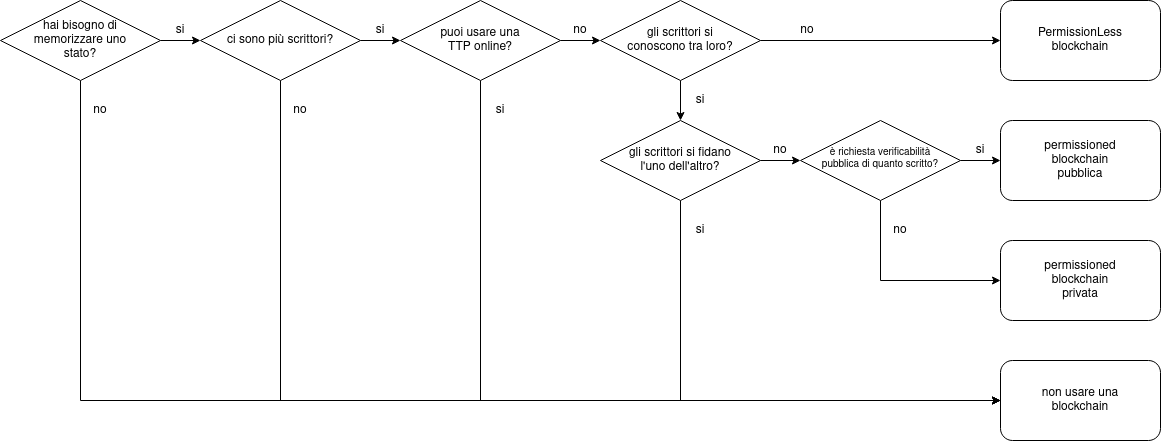
\includegraphics[scale = 0.33]{img/blockchain.png}
  \caption{Diagramma dei casi di scelta di una blockchain}
  \label{fig:bcd}
\end{figure}
\chapter{NoSQL}
Dopo aver trattato la gestione dei dati distribuita in \textbf{ambiente
  relazionale}, dopo aver trattato le blockchain anche da punto di vista di
gestione dati in \textbf{ambiente sicuro}, affrontiamo i sistemi
\textbf{NoSQL}.\\
Nel 1970 un ricercatore di IBM chiamato Codd pubblica un articolo intitolato
\textit{A relational model of data for large shared data banks} in cui presenta
un modello di rappresentazione dati indipendente dall'implementazione. Si era
passati dal \textbf{modello gerarchico} (in cui bisognava usare i puntatori per
accedere ai dati) al \textbf{modello relazionale}. Questo passaggio è stato
fondamentale per lo sviluppo del mondo dell'informatica, un mondo dove
l'hardware dedicato allo storage era estremamente costoso, estremamente poco
capiente (nel range di pochissimi megabyte) e logisticamente parecchio
ingombrante. Il modello relazionale quindi era studiato in primis per questo
contesto, proponendo strategie per la rappresentazione compatta dei dati.\\
Gli aspetti positivi del modello relazionale si possono comunque riassumere in:
\begin{itemize}
  \item è un modello molto ben definito, con il \textbf{principio della
    minimizzazione}, in merito allo spazio, e il \textbf{principio della closed
    world assumption}, ovvero tutto quello che l'applicazione deve sapere è nel
  database e a tal fine si ha anche l'uso del \texttt{NULL} \textit{value} per:
  \begin{itemize}
    \item assenza di informazione sul valore
    \item assenza di senso di un certo dato
    \item assenza di applicabilità di un certo dato
  \end{itemize}
  Quindi il modello relazionale è una sorta di \textit{modello chiuso} che
  contiene tutto il necessario ed era un modello ragionevole in un contesto come
  quello ``pre anni 2000'', dove un'azienda tipicamente necessitava solo di
  informazioni interne all'azienda stessa (non c'erano le informazioni dei
  \textit{social network} etc$\ldots$ infatti, di fatto, non esiste più la
  \textit{closed world assumption})
  \item si hanno circa 35 e più anni di sviluppo su \textit{sicurezza,
    ottimizzazione \textnormal{e} standardizzazione}. Da questo punto di vista
  si ricorda l'uso delle proprietà ACID che comunque rendono ancora valido il
  modello anche nel 2020. Inoltre ormai si hanno talmente tante informazioni
  memorizzate tramite il \textit{modello relazionale} che le aziende sono
  restie a cambiare modello (a causa dei rischi di perdita dei dati durante un
  porting, anche dati dal fatto che i db preesistenti sono enormi, considerando
  che i dati persi non sono recuperabili potenzialmente, a meno di repliche)
  \item è ben conosciuto, è studiato anche nelle scuole e nelle università
  \item è comunque la scelta migliore per diversi casi d'uso
\end{itemize}
Si hanno però anche delle limitazioni per il modello relazione, come ad esempio:
\begin{itemize}
  \item il fatto stesso di essere un \textbf{sistema chiuso}, quasi per gli
  stessi motivi descritti nei vantaggi, può anche essere un aspetto negativo,
  infatti:
  \begin{itemize}
    \item il \textbf{principio di minimizzazione}, ai giorni nostri, va a
    discapito, inutilmente, delle performance 
    \item il \textbf{principio della closed world assumption}, come già detto,
    non è praticamente più valido nell'era dei social network etc$\ldots$
    \item il modello relazionale prevede per un attributo uno e un solo valore e
    non sono quindi ammissibili array o comunque altre strutture per dati con
    multipli valori e non si possono fare interrogazioni in
    modo strutturato all'interno dei valori stessi, dovendo ricorrere a diversi
    \textit{workaround} e, secondo ``il manuale'', il metodo standard è quello
    di fare una tabella di join, detta \textit{tabella di part-of}, ovvero una
    tabella a parte coi possibili multi valori (questa soluzione porta ad
    operazioni di join molto dispendiose)
    \item non è compatibile con i linguaggi di programmazione moderni. Molti
    linguaggi moderni sono infatti OOP, con la \textit{object persistency},
    paradigma non supportato dal modello relazionale. Si hanno quindi framework
    (come \textit{Spring}) per far comunicare, tramite l'\textbf{object
      relational mapping} il modello relazionale e gli
    oggetti della OOP (aggiungendo complicazioni e perdite di
    performance). Database ad oggetti sono stati creati e implementati nei
    principali vendors ma non sono usati nelle aziende per varie ragioni, anche
    di performance e di impatto rispetto ai db relazionali
    \item non supportano i \textbf{comportamenti ciclici}, comportando limiti
    modellistici
  \end{itemize}
  \item i database relazionali sono difficili da modificare dal punto di vista
  schematico tramite \texttt{alter table}. Cambiare gli schemi è complesso e
  comporta il fermo del database
  \item per garantire le proprietà ACID nei sistemi transazionali e per poter
  garantire il 2PC si ha un limite fisico alla \textbf{scalabilità}. Dopo un
  certo punto di crescita i costi di organizzazione rendono impossibile
  l'esecuzione dei protocolli che garantiscono ACID, in ambiente
  distribuito. Oggigiorno ci sono varie applicazioni, legate in primis ai social
  network, per le quali è impossibile mantenere certi protocolli. Il problema
  della scalabilità è uno degli aspetti più limitanti, specialmente in ottica
  \textbf{big data} (anche se vedremo che le alternative non relazionali coprono
  casi d'uso anche oltre il solo ambito dei \textit{big data}). I database
  relazionali si prestano bene alle \textbf{scale up (\textit{scalabilità
      verticale})} (semplicemente aumentando
  l'hardware a disposizione, arrivando a costi esorbitanti e fino al punto in
  cui si raggiunge il limite tecnologico) ma pochissimo allo \textbf{scale out
    (\textit{scalabilità orizzontale})} (che comporterebbe non l'acquisto di un
  nuovo hardware intero ma solo di una parte di esso, a prezzo più basso con
  hardware detto in gergo \textbf{comodity},
  magari per avere più dischi etc$\ldots$, ma hardware dedicato storicamente ai
  db relazionali non prevede questa cosa). Oggigiorno si hanno sempre più spesso
  le \textbf{architetture a microservizi} (che ``implementano'' bene lo
  \textit{scale out})
  \item il \textbf{time in market}, ovvero il tempo in cui un applicativo resta
  in commercio, è sempre più ridotto (spesso, per esempio, un videogioco ha una
  vita anche inferiore ad un anno) portando a rendere obsoleto il processo in
  cui normalmente si integrano i db relazionali
\end{itemize}
Oggigiorno lo standard dal punto di vista hardware è drasticamente cambiato con
dischi di capienza enorme (nell'ordine dei terabyte per qualche decina di euro).
Il rapporto costo-gigabyte è crollato rispetto a pochi anni fa. Il contesto
storico è quindi cambiato e in tal senso anche il modello per la
rappresentazione dei dati sta cambiando e sta cambiando anche la scelta tra
\textit{spazio} e \textit{tempo}, non essendo più la prima una grossa
problematica ed essendo la seconda di grande interesse, dovendo rispondere il
più in fretta possibile alle interrogazioni.\\
\textbf{Sulle slide un elenco dei vari step storici.}
\section{I modelli NoSQL}
Il termine \textbf{NoSQL} è stato coniato da Carlo Strozzi nel 1998 quando si
inventa una sorta di API per Linux per accedere ai dati relazionali senza usare
SQL. Il termine è stato ripreso nel 2009 con la ``logica'' \textbf{Not Only
  SQL} dopo che per circa 9 anni, a partire dal 2000, erano nati nuovi modelli,
a grafi, a documenti etc$\ldots$ (da parte di Amazon, Google, Facebook
etc$\ldots$).\\
Quindi NoSQL è un'insieme di modelli di rappresentazione dati, con relativi
software di gestione. Si hanno 3 caratteristiche fondamentali:
\begin{enumerate}
  \item tutti i modello sono \textbf{schema free} o \textbf{schemaless}
  \item tutti i \textbf{DBMS NoSQL} usano il \textbf{CAP theorem}
  \item si passa da ACID a BASE (da ``acido'' a ``basico'') ovvero:
  \begin{itemize}
    \item \textit{Basic Available}
    \item \textit{Soft state}
    \item \textit{Eventual consistency}
  \end{itemize}
\end{enumerate}
\subsubsection{Schema free}
Nel modello relazionale prima veniva definito il modello, ovvero l'insieme degli
attributi che descrivevano i dati e le varie relazioni, e poi veniva popolato
con i dati veri e propri. Questo iter comportava che se durante lo sviluppo ci
si accorgeva che bisognava aggiungere, ad esempio, un attributo bisognava
modificare l'intero schema (nonché i dati già caricati). \\
Con NoSQL si è quindi passati quindi ad un'architettura dove il modello è basato
sui dati che vengono inseriti quindi di fatto per ogni ``riga'' ho
potenzialmente uno schema diverso. Questo concetto, detto \textbf{schema free}
concede una grandissima libertà di sviluppo, al costo di un'alta probabilità di
avere inconsistenza tra i dati. Si ha il cosiddetto \textbf{open word
  assumption}, dove i valori \texttt{NULL} vengono eventualmente messi solo per
motivi applicativi in quanto se un dato non c'è semplicemente non c'è e non
bisogna specificare non \texttt{NULL} il fatto che non ci sia, garantendo una
grande flessibilità (anche se questo può generare problemi). Tale flessibilità
ha comunque un costo anche dal punto di vista delle query, in quanto non si può
partire dallo schema ma si deve partire da frammenti del modello in studio. Si
ha comunque il guadagno che in caso di aggiunta di attributi etc$\ldots$ non
bisogna modificare l'intero schema, aggiungo dove serve e basta, anche se
ovviamente serve una \textit{governance} del dato più forte (in quanto può anche
succedere che non si abbia il tipo di dato). 
\subsubsection{CAP theorem}
Vediamo questo teorema essenziale\footnote{così L.T. è contento}, proposto da
Gilber e Lynch nel 2002 dopo che, qualche anno prima, nel 2000, Brewer aveva
proposto una sua \textit{congettura sulla consistenza, disponibilità e
  partizionamento dei webserver}. Il teorema dimostra la congettura di Brewer:
\begin{teorema}[CAP theorem]
  Preso un \textbf{sistema distribuito di nodi} si considerino tre aspetti:
  \begin{itemize}
    \item \textbf{Consistency (\textit{consistenza})}, ovvero che tutti i nodi
    abbaino gli stessi i dati nello stesso istante (che è diverso dalla
    consistenza di ACID)
    \item \textbf{Availability (\textit{disponibilità})}, ovvero la garanzia che
    ogni richiesta ricevuta da un sistema riceva una risposta in
    ogni caso, sia in caso fallimento che successo (non si deve avere quindi
    un'attesa infinita)
    \item \textbf{Partition tolerance (\textit{partizionamento})}, ovvero il
    sistema deve continuare ad operare comunque anche se si hanno perdite di
    messaggi o fallimenti di parti del sistema
  \end{itemize}
  Il teorema garantisce che tra queste tre caratteristiche, in un sistema
  distribuito, se ne possano avere contemporaneamente due soddisfatte e mai tre.
\end{teorema}
Si nota quindi come, prendendo ad esempio i DDBMS, si rinunci alla
\textit{partition tolerance}, garantendo le prime due caratteristiche (anche se
con un numero limitato di nodi si può arrivare ad una buona resa anche dal
punto di vista della \textit{partition tolerance}).\\
I sistemi NoSQL tipicamente divisi tra:
\begin{itemize}
  \item sistemi che garantiscono \textit{consistency} e \textit{partition
    tolerance} (CP), non potendo garantire che il DBMS lavori 24/7. Tra questi
  troviamo:
  \textit{BigTable, Hypertable, HBase, MongoDB, Terrastore, Scalaris, Berkeley
    DB, MemcacheDB, Redis $\ldots$}
  \item sistemi che garantiscono \textit{availability} e \textit{partition
    tolerance} (AP), non potendo garantire che i dati siano sempre
  consistenti. Tra questi troviamo: \textit{Dynamo, Voldemort, Tokyo Cabinet,
    KAI, Cassandra, SimpleDB, CouchDB Riak $\ldots$}
\end{itemize}
Non è detto che due db NoSQL che implementano lo stesso modello, ad esempio
documentale, garantiscano le stesse due caratteristiche CAP.\\
Quindi in fase progettuale la scelta tra due delle caratteristiche CAP è un
punto chiave per poi scegliere eventualmente su che DBMS NoSQL appoggiarsi (o
anche partire da un DBMS NoSQL che già si conosce ma essendo consci della
caratteristica non garantita).\\
Ci sono contesti applicativi in cui ognuna delle tre caratteristiche può, a
seconda, non essere fondamentale. In ogni caso si ha che:
\begin{itemize}
  \item \textit{consistency} mi garantisce che tutti i client hanno sempre la
  stessa vista sui dati
  \item \textit{availability} mi garantisce che ogni client può sempre leggere
  e/o scrivere
  \item \textit{partition tolerance} mi garantisce che il sistema continui a
  funzionare nonostante partizioni fisiche della rete
\end{itemize}
In fase progettuale quindi ho 3 step:
\begin{itemize}
  \item scelta del modello
  \item scelta del DBMS
  \item scelta delle caratteristiche del CAP theorem
\end{itemize}
\subsubsection{BASE}
Analizziamo meglio l'acronimo.
\begin{itemize}
  \item \textit{Basic Available}, ovvero, comunque vada, la risposta viene
  sempre data anche nel caso di consistenza parziale
  \item \textit{Soft state}, ovvero si rinuncia al concetto di consistenza di
  ACID
  \item \textit{Eventual consistency}, ovvero, ad un certo punto prima o poi
  nel futuro (magari anche dopo pochissimi secondi),
  i dati ``convergeranno'' ad uno stato di consistenza (in opposizione alla
  consistenza immediata di ACID)
\end{itemize}
Vediamo quindi i vari modelli NoSQL:
\begin{itemize}
  \item \textbf{key-value stores} (come \textit{Dynamo, Voldemort, Redis, Riak
    $ldots$}) che è il modello più semplice. È infatti il semplice modello
  \textit{chiave-valore}, semplice da memorizzare, e utile per il caching. Il
  valore è un \textit{blob} quindi non si ha modo di interrogare internamente il
  valore me deve essere l'applicazione a manipolarlo. La chiave garantisce
  tipicamente meccanismi di hash, con la chiave che punta ad un certo
  valore, massimizzando le performance. Viene garantito l'\textit{hashing
    distribuito}, ovvero la \textit{distributed hashed table}
  \item \textbf{column family stores}, (come
  \textit{BigTable, Cassandra, HBase $\ldots$}) dove la chiave punta a colonne
  multiple di valori, ottenendo un formato \textit{pseudo-relazione}. Ogni riga,
  in questo schema \textbf{wide column}, ha una sua struttura interna diversa a
  quella di altre righe, che sono comunque indipendenti. La chiave ovviamente
  può essere hashata. Non posso fare \textit{ranged query}
  \item \textbf{document databases} (come \textit{CouchDB, MongoDB $\ldots$}) è
  formato da documenti con coppie chiave-valore o chiave-oggetto, dove l'oggetto
  può anche essere un'altra chiave-valore, un array di valori, un array di
  oggetti etc$\ldots$. Un esempio pratico di documento è il tipico file json,
  che è ottimo per dire che nel modello documentale si ha un elemento più
  importante, detto \textit{root} che ha al di sotto tutti gli altri
  \item \textbf{graph databases} (come \textit{Neo4J, FlockDB, GraphBase,
    InfoGrip $\ldots$}) con nodi e relazioni tra gli stessi rappresentate dagli
  archi. I nodi possono rappresentare entità a cui sono associate varie
  proprietà (e si chiamano \textit{property graph}). le proprietà sono quindi
  pertinenti ai nodi. I graph db non scalano bene
  \item \textbf{RDF databases}
\end{itemize}
(\textit{Spesso l'azienda stessa non è attenta al tipo di modello usato quindi
  si hanno spesso confusioni}).\\
A livello di complessità (anche dei dati che rappresentano) possiamo dire che,
seguendo l'ordine elencato, si passa dal più semplice al più complesso. Anche
dal punto di vista del volume abbiamo lo stesso ordine, dal più voluminoso
(quindi il meno complesso è anche il più voluminoso ma più scalabile) a quello
meno voluminoso e scalabile.\\
Il problema fondamentale in tutti questi modelli è come connettere le
informazioni e questo diventa un problema fondamentale in termini di prestazioni
e analisi da effettuare. Si ha che le relazioni sono implicitamente incluse nei
dati. La scelta del modello dipende dall'applicativo e ci sono applicativi che
possono obbligare ad avere due o più modelli.\\
Ovviamente ogni vendor ha il suo linguaggio di query per il suo DBMS NoSQL.
\end{document}
% LocalWords:  Machine Learning DBMS DataBase System hashmap db workload system
% LocalWords:  storage Administrator DBA GUI SPARC performanti primis query SQL
% LocalWords:  join compiler DLL DDL Language step parsing Catalog metadati sql
% LocalWords:  tree parser plan select sottotabella FROM Where Stafford mgrssn
% LocalWords:  Bdate Pnumber l'ottimizzatore where Statistics Branch Bound work
% LocalWords:  transaction begin commit rollabck OLTP OnLine Processing ACID PL
% LocalWords:  rollback UNDO recovery serializzabile conflict equivalence locks
% LocalWords:  two phase locking shared deadlock timestamps lock serializzabili
% LocalWords:  unlock nothing vendor cloud DDBMS l'ottimizzatore Peer to client
% LocalWords:  object oriented OO example json warehouse LAV Local As View ODBC
% LocalWords:  routing processing vendors middleware DTP Distributed devices TM
% LocalWords:  GRID warehouses everything SMP Oracle RAC systems performances
% LocalWords:  big sottotabelle soft fail chunk ricostruibilità l'updates local
% LocalWords:  l'updates mapping rewriting replication decomposition global dur
% LocalWords:  optimization localization send receive semijoin runtime layer LM
% LocalWords:  monitoring response setup bytes gigabit throughput AssiGN eno RM
% LocalWords:  ename resp sse l'updates LocalWords l'updates fragment dell read
% LocalWords:  requests only transactions write insert update distribuited All
% LocalWords:  ottimizzatore reliability control concurrency schedules ROWA RPC
% LocalWords:  serializzabilità items primary copy stricted centralized wait of
% LocalWords:  Call external slide PDF ack abort resource managers log RMs not
% LocalWords:  prepare ready checkpoint dump img png decision recoverable all
% LocalWords:  records failure broadcast warm restart undo presumed xopen TX XA
% LocalWords:  interface IBM Microsoft technologies realtime based snapshot and
% LocalWords:  transactional merge over loss disaster mission critical load OOP
% LocalWords:  kilometri consolidation distribution balancing offline entry BTC
% LocalWords:  reporting warehousing commerce social testing compliant many GB
% LocalWords:  source directional resolution detention Tier staging event apply
% LocalWords:  publish publisher distributor subscriber intra inter paradigm js
% LocalWords:  relational mismatch Blockchain mapper Delete framework group SHA
% LocalWords:  multicore Blockchains blockchain bitcoin criptovalute genesis
% LocalWords:  block hash torrent double spanning Leporati ethereum monero spam
% LocalWords:  zcash foreniscs criptovaluta Satoshi Nakamoto paper proof part
% LocalWords:  spending bitcoins wallet miners Moore RIPEMD iniettiva one way
% LocalWords:  nonce miner mining farm stake fee blockchains ether ETH smart
% LocalWords:  contract Solidity struct function bytecode virtual machine remix
% LocalWords:  outOfGas OpenZeppelin startup overflow metamask l'ide Rapsten
% LocalWords:  Rinkeby autority Truffle Ganache main MetaMask webapp GoQuorum
% LocalWords:  permission permissionless third TTP permissioned audit Chaos EOS
% LocalWords:  webassembly Hyperledger authority Foundation SAP CryptoKitties
% LocalWords:  collezzionabili NoSQL for large banks Codd logisticamente closed
% LocalWords:  terabyte gigabyte world assumption NULL value pre porting array
% LocalWords:  workaround persistency table comodity microservizi Amazon Google
% LocalWords:  Facebook schemaless CAP theorem Basic Available Eventually Lynch
% LocalWords:  consistency governance Brewer webserver Gilber Availability key
% LocalWords:  Partition partition availability Eventual stores column family
% LocalWords:  document databases graph RDF tuple caching blob hashing hashed
% LocalWords:  distributed wide hashata ranged property root
